
\chapter{Important à savoir}
\section{Pourquoi à partir des temps RTTs bruts on arrive à détecter les anomalies?}


La détection des anomalies se base sur la caractérisation de la distribution des RTTs différentiels. Tel que dans un premier temps, on construise une référence et ensuite identifier les déviation par rapport à cette référence.


En pratique, la détection des anomalies repose sur une variante du théorème central limite (CLT).

Dans notre cas, la distribution des moyennes d'un nombre assez large d'échantillons des RTTs différentiels sont distribuées normalement. En cas de changement du délai entre les deux routeurs X et Y, la moyenne résultante dévie de la distribution normale ainsi une anomalie est détectée.


Les premières expériences ont montré que les valeurs "bruits" peuvent affecter largement les valeurs des moyennes calculées d'où la nécessité d'avoir un nombre très important d'échantillons, ce qui est n'est pas praticable. Afin de résoudre ce besoin, les autres du travail ont utilisé la médiane à la place de la moyenne car :

\begin{itemize}
	\item elle est robuste aux valeurs bruits des RTTs;
	\item la convergence des médianes vers la distribution normale nécessite moins d'échantillons. 
\end{itemize}


\section{Rappel}
La programmation fonctionnelle est parmi les paradigmes de programmation.  Ce paradigme se base sur les fonctions au sens mathématique du terme.
 
 \section{Processus de détection des anomalies}
 \subsection{Les phases de la détection }
 \paragraph{Phase I : préparation des données}
 La Figure D.1 reprend les étapes de la phase I. Chaque étape est définie par ses entrées et
 ses sorties. L’objectif de chaque étape est détaillé dans ce qui suit :
 \begin{itemize}
 	\item \textbf{findAllBins (I.1)} : nous cherchons toutes périodes {\color{gray}([bin])} entre start et end dont leur
 durée est de timeWindow.
 \item \textbf{findTraceroutesByBin (I.2)} : pour toute période  {\color{gray}bin}, nous récupérons les traceroutes
 capturés durant cette dernière. Le nombre de traceroutes associés à chaque bin dépend
 des traceroutes disponibles à l’analyse  {\color{gray}([traceroute])}.
 \item \textbf{aggregateRttsByHop (I.3)} : certains traceroutes ne réussissent pas à atteindre la destina-
 tion prévue. Dans ce cas, ces traceroutes sont ignorés. Les saut ayant des RTTs invalides
 sont aussi ignorés.
 \item \textbf{aggregateRttsByHop (I.4)} : étant donné que chaque saut  {\color{gray}(hop)} est décrit par plus d’un
 RTT, nous calculons la médiane de ces RTTs  {\color{gray}(rttAgg)}, et ce par source de signal.
 \item \textbf{linkInference (I.5)} : chaque deux sauts consécutifs d’un traceroute forment un lien. Pour
 tout traceroute d’un bin donné, nous inférons les liens possibles. Ensuite, nous caractérisons ce lien  {\color{gray}(ip1, ip2)} avec son RTT différentiel  {\color{gray}(rttDiff)}.
\item \textbf{sortLinks (I.6) }: à cette étape, nous ordonnons les couples d'adresses IP  {\color{gray}(ip1, ip2)} suivant l'ordre alphabétique. Par exemple, 
 
 \item \textbf{mergeLinks (I.7)} : nous fusionnons les liens avec leurs caractéristiques. En résultat, les
 liens (ip1, ip2) et (ip2, ip1) sont fusionnés et sont représentés par le lien (ip1, ip2) si (ip1,
 ip2) < (ip2, ip1).
 \item \textbf{resumeData (1.8)} : jusqu’à cette étape, les liens sont organisés par bin. Vu qu’un lien
 peut être identifié durant plusieurs périodes, nous résumons un lien en fusionnant leurs
 RTTs différentiels. Toutefois, chaque RTT différentiel doit garder le bin pendant lequel il
 a été identifié, ainsi les deux listes  {\color{gray}[rttDiff]} et  {\color{gray}[bin]} ont la même longueur.
 
 
\end{itemize}

\paragraph{ Phase II : détection des anomalies}

 A la fin de la phase I, nous avons à notre disposition tous les liens identifiés avec leurs
 caractéristiques. La Figure D.2 illustre les étapes principales de la phase II.
 
 \begin{itemize}

 \item \textbf{ findAllBins (II.1)} : nous générons les mêmes périodes  {\color{gray}(bin)} que celles générées dans
 l'étape (I.1).
 \item \textbf{ findRTTDiffByBin (II.2)} : nous reprenons les périodes dans l'ordre chronologique et
 pour chaque bin nous cherchons les RTTs différentiels correspondants à chaque  {\color{gray}bin}. Nous
 notons  {\color{gray}(dist)} l'ensemble des RTTs différentiels correspondants à un bin donné.
 Note : La période ayant enregistré moins de 4 RTTs différentiels est négligée et nous
 passons à la période suivante.
\item \textbf{ wilsonScoreProcess (II.3)} : le calcul de l'interface de confiance à partir du score de Wilson nécessite d'avoir le nombre total des expériences, le nombre d'expérience réussies et  le risque d'erreur. Nous calculons les deux bornes du score de Wilson suivant les étapes suivantes :

\begin{enumerate}
	\item Soit $n$ la taille de la distribution, nous calculons le score de Wilson, ce que donne le couple de valeurs ($ low $, $ hight $).
	\item nous multiplions $ low $ et $ hight $ par  $n$, ainsi nous avons ( $ lo $, $ hi $ )=  ($ n*low $, $ n*hight $).
	\item nous récupérons la partie entière du  $ lo $ et $ hi $, ainsi nous avons ( $l$, $h$) = ($ int $($ lo $), $ int $($ hi $))\footnote{La fonction $  int() $ est utilisée pour avoir la partie entière d'un nombre.}.
	\item  nous parcourons la distribution {\color{gray}{dist}} pour trouver les RTTs différentiels qui se trouvent au rang $  l $ et $ h $ dans {\color{gray}dist}, respectivement sont $ rttDiffL $, $ rttDiffH $. Ainsi :
	
	 $ rttDiffL $ = dist[l]  et $ rttDiffH$ = dist[h], avec l, h $\in$ $[0,n[$. 
	
\end{enumerate}


 \item \textbf{updateCurrentLinkState (II.4)} :  {\color{gray}current}  est l'état courant du lien à une période donnée.  Nous calculons l'état du lien en ce bin en calculant:
 
 \begin{itemize}[label=$\square$]
 	\item le RTT différentiel médian ({\color{gray}median}) pour le bin courant.
 	
 	{\color{gray}currentMedian} = median(dist) 
 	
 	\item  la borne inférieure de l'intervalle de confiance ({\color{gray}ciLow})
 	
 	{\color{gray}currentCiLow} = {\color{gray}median} --  $ rttDiffL $
 	
 	\item   la borne supérieure de l'intervalle de confiance ({\color{gray}ciHight}).
 	
 	{\color{gray}currentCiHight} =  $ rttDiffH$ --  {\color{gray}median}
 	
 \end{itemize}

\item \textbf{ updateReferenceLinkState(II.5)} :  {\color{gray}reference}  est l'état de référence du lien à une période donnée. Son calcul est réalisé selon trois cas. De même que l'état courant, l'état référence est décrit par la médiane du RTT différentiel, la borne inférieure de l'intervalle de confiance de référence et enfin la borne supérieure de l'intervalle de confiance de référence.

\begin{enumerate}
	\item Tant que nous n'avons pas construit une référence assez représentable de l'état du lien (cas 1).  nous mettons à jour la référence ({reference}) comme suit: 
	
	referenceMedian = median(dist)
	
	referenceCiLow = rttDiffL
	
	referenceCiHight = rttDiffH
	
	\item Une fois nous atteignons le nombre nécessaire de  mise à jour de la référence assurant la représentativité de la référence (cas 2), nous mettons à jour l'état référence en remplaçant la médiane de chaque période par aggre\_median, la borne inférieure  de chaque période par  aggr\_ciLow et la borne sépérieure de chaque période par aggr\_ciHigh.
	\begin{itemize}
		
\item  soit aggre\_median la médiane de tous les RTTs différentiels médians de référence calculés pour toutes les périodes précédentes. 
	
\item 	soit aggr\_ciLow la médiane de tous les   toutes les bornes inférieures calculées pendant les périodes précédentes.
	
\item 	soit aggr\_ciHigh la médiane de tous les   toutes les bornes inférieures calculées pendant les périodes précédentes.

\end{itemize}

	
	\item Une fois la référence est représentable (cas 3), nous mettons à jour cette dernière comme suit :
	
		referenceMedian = $  0.99*referenceMedian[-1]+0.01*currentMedian $
	
		 referenceCiLow =	$ 0.99*referenceLow[-1]+0.01*rttDiffL $
		 
	referenceCiHight = $ 0.99*referenceHight[-1]+0.01*rttDiffH $
	

	   
	

\end{enumerate}
 \item \textbf{ alarmsDetection (II.6) }:   la détection des anomalies est déclenché à partir du cas 3. Si une anomalie est détectée, nous mettons à jour la liste des alarmes  {\color{gray}(alarmsValues)} avec le RTT différentiel médian (currentMedian) ainsi que la
 liste des dates  {\color{gray}(alarmsDates)} qui correspondent à ces anomalies. Les anomalies sont détecté en évaluant le chevauchement entre l'intervalle de confiance courant et celui de référence. La période courante présente une anomalie si la condition suivante est vraie\footnote{Nous notons par [-1] l'élément précédent d'une mesure. Par exemple, currentMedian[-1] est la médiane des RTTs différentiels de la période qui précède la période courante.}:
 \begin{lstlisting}[language=json,firstnumber=1, caption={Illustration},
 basicstyle =\footnotesize]
currentMedian[-1]-currentCiLow[-1] > referenceHi[-1] or
currentMedian[-1]+currentCiHigh[-1] < referenceCiLow[-1]) and
np.abs(currentMedian[-1]-reference[-1])>1
 \end{lstlisting}

 
 
  \end{itemize}

\paragraph{ Illustrations des deux phases de détection}~
\newpage

\begin{figure}[H]
	\centering
	\captionsetup{justification=centering}
	\resizebox{!}{\textheight}{
		% Graphic for TeX using PGF
% Title: /home/hayat/RipeAtlasTraceroutesAnalysis/2019/Rapport_Mai/illustrations/step-preparing-data.dia
% Creator: Dia v0.97+git
% CreationDate: Wed May 22 04:23:28 2019
% For: hayat
% \usepackage{tikz}
% The following commands are not supported in PSTricks at present
% We define them conditionally, so when they are implemented,
% this pgf file will use them.
\ifx\du\undefined
  \newlength{\du}
\fi
\setlength{\du}{15\unitlength}
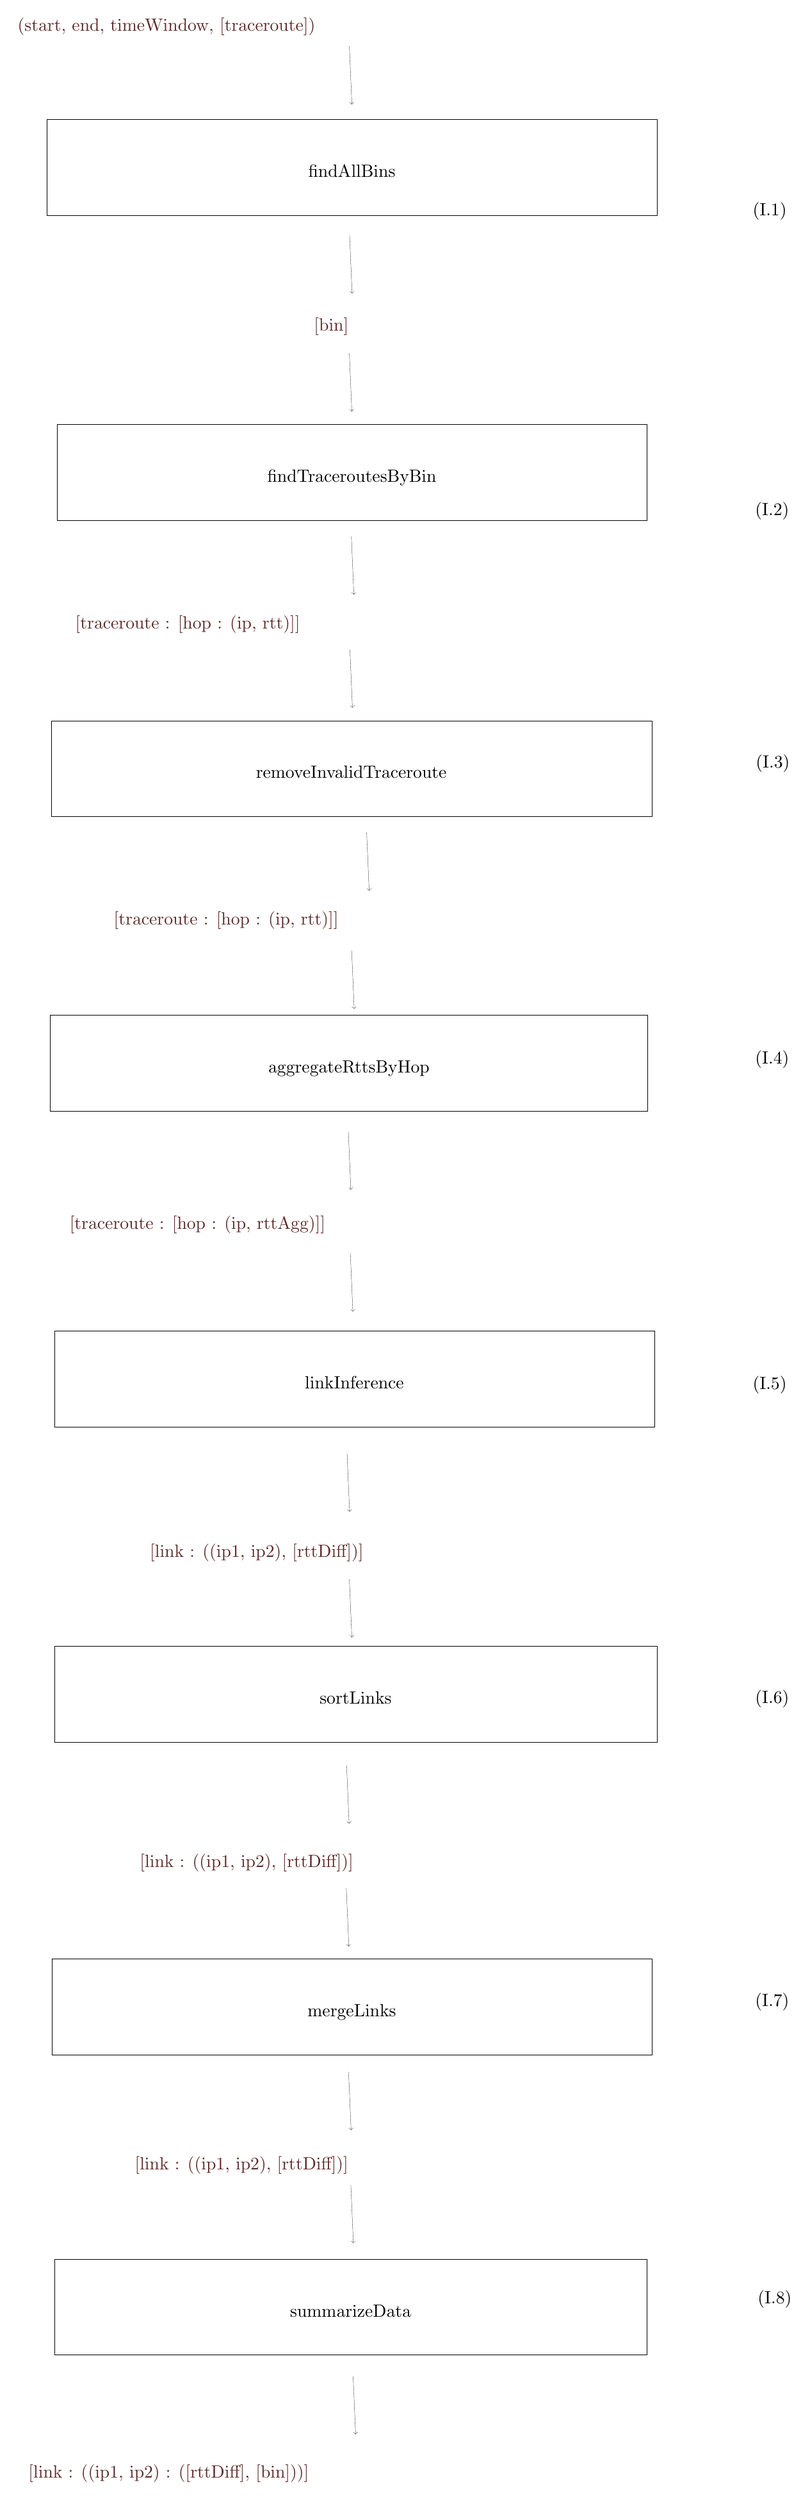
\begin{tikzpicture}[even odd rule]
\pgftransformxscale{1.000000}
\pgftransformyscale{-1.000000}
\definecolor{dialinecolor}{rgb}{0.000000, 0.000000, 0.000000}
\pgfsetstrokecolor{dialinecolor}
\pgfsetstrokeopacity{1.000000}
\definecolor{diafillcolor}{rgb}{1.000000, 1.000000, 1.000000}
\pgfsetfillcolor{diafillcolor}
\pgfsetfillopacity{1.000000}
\pgfsetlinewidth{0.100000\du}
\pgfsetdash{}{0pt}
\pgfsetmiterjoin
{\pgfsetcornersarced{\pgfpoint{0.000000\du}{0.000000\du}}\definecolor{diafillcolor}{rgb}{1.000000, 1.000000, 1.000000}
\pgfsetfillcolor{diafillcolor}
\pgfsetfillopacity{1.000000}
\fill (14.000000\du,1.586360\du)--(14.000000\du,3.486360\du)--(26.100000\du,3.486360\du)--(26.100000\du,1.586360\du)--cycle;
}{\pgfsetcornersarced{\pgfpoint{0.000000\du}{0.000000\du}}\definecolor{dialinecolor}{rgb}{0.000000, 0.000000, 0.000000}
\pgfsetstrokecolor{dialinecolor}
\pgfsetstrokeopacity{1.000000}
\draw (14.000000\du,1.586360\du)--(14.000000\du,3.486360\du)--(26.100000\du,3.486360\du)--(26.100000\du,1.586360\du)--cycle;
}% setfont left to latex
\definecolor{dialinecolor}{rgb}{0.000000, 0.000000, 0.000000}
\pgfsetstrokecolor{dialinecolor}
\pgfsetstrokeopacity{1.000000}
\definecolor{diafillcolor}{rgb}{0.000000, 0.000000, 0.000000}
\pgfsetfillcolor{diafillcolor}
\pgfsetfillopacity{1.000000}
\node[anchor=base,inner sep=0pt, outer sep=0pt,color=dialinecolor] at (20.050000\du,2.731360\du){findAllBins};
% setfont left to latex
\definecolor{dialinecolor}{rgb}{0.360784, 0.152941, 0.152941}
\pgfsetstrokecolor{dialinecolor}
\pgfsetstrokeopacity{1.000000}
\definecolor{diafillcolor}{rgb}{0.360784, 0.152941, 0.152941}
\pgfsetfillcolor{diafillcolor}
\pgfsetfillopacity{1.000000}
\node[anchor=base west,inner sep=0pt,outer sep=0pt,color=dialinecolor] at (13.422300\du,-0.163641\du){(start, end, timeWindow, \ensuremath{[}traceroute\ensuremath{]})};
\pgfsetlinewidth{0.100000\du}
\pgfsetdash{}{0pt}
\pgfsetbuttcap
{
\definecolor{diafillcolor}{rgb}{0.000000, 0.000000, 0.000000}
\pgfsetfillcolor{diafillcolor}
\pgfsetfillopacity{1.000000}
% was here!!!
\pgfsetarrowsend{to}
\definecolor{dialinecolor}{rgb}{0.000000, 0.000000, 0.000000}
\pgfsetstrokecolor{dialinecolor}
\pgfsetstrokeopacity{1.000000}
\draw (20.000000\du,0.136359\du)--(20.050000\du,1.291360\du);
}
% setfont left to latex
\definecolor{dialinecolor}{rgb}{0.360784, 0.152941, 0.152941}
\pgfsetstrokecolor{dialinecolor}
\pgfsetstrokeopacity{1.000000}
\definecolor{diafillcolor}{rgb}{0.360784, 0.152941, 0.152941}
\pgfsetfillcolor{diafillcolor}
\pgfsetfillopacity{1.000000}
\node[anchor=base west,inner sep=0pt,outer sep=0pt,color=dialinecolor] at (19.300000\du,5.786360\du){\ensuremath{[}bin\ensuremath{]}};
\pgfsetlinewidth{0.100000\du}
\pgfsetdash{}{0pt}
\pgfsetmiterjoin
{\pgfsetcornersarced{\pgfpoint{0.000000\du}{0.000000\du}}\definecolor{diafillcolor}{rgb}{1.000000, 1.000000, 1.000000}
\pgfsetfillcolor{diafillcolor}
\pgfsetfillopacity{1.000000}
\fill (14.200000\du,7.636360\du)--(14.200000\du,9.536360\du)--(25.900000\du,9.536360\du)--(25.900000\du,7.636360\du)--cycle;
}{\pgfsetcornersarced{\pgfpoint{0.000000\du}{0.000000\du}}\definecolor{dialinecolor}{rgb}{0.000000, 0.000000, 0.000000}
\pgfsetstrokecolor{dialinecolor}
\pgfsetstrokeopacity{1.000000}
\draw (14.200000\du,7.636360\du)--(14.200000\du,9.536360\du)--(25.900000\du,9.536360\du)--(25.900000\du,7.636360\du)--cycle;
}% setfont left to latex
\definecolor{dialinecolor}{rgb}{0.000000, 0.000000, 0.000000}
\pgfsetstrokecolor{dialinecolor}
\pgfsetstrokeopacity{1.000000}
\definecolor{diafillcolor}{rgb}{0.000000, 0.000000, 0.000000}
\pgfsetfillcolor{diafillcolor}
\pgfsetfillopacity{1.000000}
\node[anchor=base,inner sep=0pt, outer sep=0pt,color=dialinecolor] at (20.050000\du,8.781360\du){findTraceroutesByBin};
% setfont left to latex
\definecolor{dialinecolor}{rgb}{0.360784, 0.152941, 0.152941}
\pgfsetstrokecolor{dialinecolor}
\pgfsetstrokeopacity{1.000000}
\definecolor{diafillcolor}{rgb}{0.360784, 0.152941, 0.152941}
\pgfsetfillcolor{diafillcolor}
\pgfsetfillopacity{1.000000}
\node[anchor=base west,inner sep=0pt,outer sep=0pt,color=dialinecolor] at (14.565900\du,11.686400\du){\ensuremath{[}traceroute : \ensuremath{[}hop : (ip, rtt)\ensuremath{]}\ensuremath{]}};
\pgfsetlinewidth{0.100000\du}
\pgfsetdash{}{0pt}
\pgfsetmiterjoin
{\pgfsetcornersarced{\pgfpoint{0.000000\du}{0.000000\du}}\definecolor{diafillcolor}{rgb}{1.000000, 1.000000, 1.000000}
\pgfsetfillcolor{diafillcolor}
\pgfsetfillopacity{1.000000}
\fill (14.066600\du,19.341700\du)--(14.066600\du,21.241700\du)--(25.916600\du,21.241700\du)--(25.916600\du,19.341700\du)--cycle;
}{\pgfsetcornersarced{\pgfpoint{0.000000\du}{0.000000\du}}\definecolor{dialinecolor}{rgb}{0.000000, 0.000000, 0.000000}
\pgfsetstrokecolor{dialinecolor}
\pgfsetstrokeopacity{1.000000}
\draw (14.066600\du,19.341700\du)--(14.066600\du,21.241700\du)--(25.916600\du,21.241700\du)--(25.916600\du,19.341700\du)--cycle;
}% setfont left to latex
\definecolor{dialinecolor}{rgb}{0.000000, 0.000000, 0.000000}
\pgfsetstrokecolor{dialinecolor}
\pgfsetstrokeopacity{1.000000}
\definecolor{diafillcolor}{rgb}{0.000000, 0.000000, 0.000000}
\pgfsetfillcolor{diafillcolor}
\pgfsetfillopacity{1.000000}
\node[anchor=base,inner sep=0pt, outer sep=0pt,color=dialinecolor] at (19.991600\du,20.486700\du){aggregateRttsByHop};
% setfont left to latex
\definecolor{dialinecolor}{rgb}{0.360784, 0.152941, 0.152941}
\pgfsetstrokecolor{dialinecolor}
\pgfsetstrokeopacity{1.000000}
\definecolor{diafillcolor}{rgb}{0.360784, 0.152941, 0.152941}
\pgfsetfillcolor{diafillcolor}
\pgfsetfillopacity{1.000000}
\node[anchor=base west,inner sep=0pt,outer sep=0pt,color=dialinecolor] at (14.452400\du,23.585000\du){\ensuremath{[}traceroute : \ensuremath{[}hop : (ip, rttAgg)\ensuremath{]}\ensuremath{]}};
\pgfsetlinewidth{0.100000\du}
\pgfsetdash{}{0pt}
\pgfsetmiterjoin
{\pgfsetcornersarced{\pgfpoint{0.000000\du}{0.000000\du}}\definecolor{diafillcolor}{rgb}{1.000000, 1.000000, 1.000000}
\pgfsetfillcolor{diafillcolor}
\pgfsetfillopacity{1.000000}
\fill (14.150000\du,25.600000\du)--(14.150000\du,27.500000\du)--(26.050000\du,27.500000\du)--(26.050000\du,25.600000\du)--cycle;
}{\pgfsetcornersarced{\pgfpoint{0.000000\du}{0.000000\du}}\definecolor{dialinecolor}{rgb}{0.000000, 0.000000, 0.000000}
\pgfsetstrokecolor{dialinecolor}
\pgfsetstrokeopacity{1.000000}
\draw (14.150000\du,25.600000\du)--(14.150000\du,27.500000\du)--(26.050000\du,27.500000\du)--(26.050000\du,25.600000\du)--cycle;
}% setfont left to latex
\definecolor{dialinecolor}{rgb}{0.000000, 0.000000, 0.000000}
\pgfsetstrokecolor{dialinecolor}
\pgfsetstrokeopacity{1.000000}
\definecolor{diafillcolor}{rgb}{0.000000, 0.000000, 0.000000}
\pgfsetfillcolor{diafillcolor}
\pgfsetfillopacity{1.000000}
\node[anchor=base,inner sep=0pt, outer sep=0pt,color=dialinecolor] at (20.100000\du,26.745000\du){linkInference};
% setfont left to latex
\definecolor{dialinecolor}{rgb}{0.360784, 0.152941, 0.152941}
\pgfsetstrokecolor{dialinecolor}
\pgfsetstrokeopacity{1.000000}
\definecolor{diafillcolor}{rgb}{0.360784, 0.152941, 0.152941}
\pgfsetfillcolor{diafillcolor}
\pgfsetfillopacity{1.000000}
\node[anchor=base west,inner sep=0pt,outer sep=0pt,color=dialinecolor] at (16.045000\du,30.085000\du){\ensuremath{[}link : ((ip1, ip2), \ensuremath{[}rttDiff\ensuremath{]})\ensuremath{]}};
\pgfsetlinewidth{0.100000\du}
\pgfsetdash{}{0pt}
\pgfsetmiterjoin
{\pgfsetcornersarced{\pgfpoint{0.000000\du}{0.000000\du}}\definecolor{diafillcolor}{rgb}{1.000000, 1.000000, 1.000000}
\pgfsetfillcolor{diafillcolor}
\pgfsetfillopacity{1.000000}
\fill (14.150000\du,31.850000\du)--(14.150000\du,33.750000\du)--(26.100000\du,33.750000\du)--(26.100000\du,31.850000\du)--cycle;
}{\pgfsetcornersarced{\pgfpoint{0.000000\du}{0.000000\du}}\definecolor{dialinecolor}{rgb}{0.000000, 0.000000, 0.000000}
\pgfsetstrokecolor{dialinecolor}
\pgfsetstrokeopacity{1.000000}
\draw (14.150000\du,31.850000\du)--(14.150000\du,33.750000\du)--(26.100000\du,33.750000\du)--(26.100000\du,31.850000\du)--cycle;
}% setfont left to latex
\definecolor{dialinecolor}{rgb}{0.000000, 0.000000, 0.000000}
\pgfsetstrokecolor{dialinecolor}
\pgfsetstrokeopacity{1.000000}
\definecolor{diafillcolor}{rgb}{0.000000, 0.000000, 0.000000}
\pgfsetfillcolor{diafillcolor}
\pgfsetfillopacity{1.000000}
\node[anchor=base,inner sep=0pt, outer sep=0pt,color=dialinecolor] at (20.125000\du,32.995000\du){sortLinks};
% setfont left to latex
\definecolor{dialinecolor}{rgb}{0.360784, 0.152941, 0.152941}
\pgfsetstrokecolor{dialinecolor}
\pgfsetstrokeopacity{1.000000}
\definecolor{diafillcolor}{rgb}{0.360784, 0.152941, 0.152941}
\pgfsetfillcolor{diafillcolor}
\pgfsetfillopacity{1.000000}
\node[anchor=base west,inner sep=0pt,outer sep=0pt,color=dialinecolor] at (15.845000\du,36.235000\du){\ensuremath{[}link : ((ip1, ip2), \ensuremath{[}rttDiff\ensuremath{]})\ensuremath{]}};
\pgfsetlinewidth{0.100000\du}
\pgfsetdash{}{0pt}
\pgfsetmiterjoin
{\pgfsetcornersarced{\pgfpoint{0.000000\du}{0.000000\du}}\definecolor{diafillcolor}{rgb}{1.000000, 1.000000, 1.000000}
\pgfsetfillcolor{diafillcolor}
\pgfsetfillopacity{1.000000}
\fill (14.100000\du,38.050000\du)--(14.100000\du,39.950000\du)--(26.000000\du,39.950000\du)--(26.000000\du,38.050000\du)--cycle;
}{\pgfsetcornersarced{\pgfpoint{0.000000\du}{0.000000\du}}\definecolor{dialinecolor}{rgb}{0.000000, 0.000000, 0.000000}
\pgfsetstrokecolor{dialinecolor}
\pgfsetstrokeopacity{1.000000}
\draw (14.100000\du,38.050000\du)--(14.100000\du,39.950000\du)--(26.000000\du,39.950000\du)--(26.000000\du,38.050000\du)--cycle;
}% setfont left to latex
\definecolor{dialinecolor}{rgb}{0.000000, 0.000000, 0.000000}
\pgfsetstrokecolor{dialinecolor}
\pgfsetstrokeopacity{1.000000}
\definecolor{diafillcolor}{rgb}{0.000000, 0.000000, 0.000000}
\pgfsetfillcolor{diafillcolor}
\pgfsetfillopacity{1.000000}
\node[anchor=base,inner sep=0pt, outer sep=0pt,color=dialinecolor] at (20.050000\du,39.195000\du){mergeLinks};
% setfont left to latex
\definecolor{dialinecolor}{rgb}{0.360784, 0.152941, 0.152941}
\pgfsetstrokecolor{dialinecolor}
\pgfsetstrokeopacity{1.000000}
\definecolor{diafillcolor}{rgb}{0.360784, 0.152941, 0.152941}
\pgfsetfillcolor{diafillcolor}
\pgfsetfillopacity{1.000000}
\node[anchor=base west,inner sep=0pt,outer sep=0pt,color=dialinecolor] at (15.745000\du,42.235000\du){\ensuremath{[}link : ((ip1, ip2), \ensuremath{[}rttDiff\ensuremath{]})\ensuremath{]}};
\pgfsetlinewidth{0.100000\du}
\pgfsetdash{}{0pt}
\pgfsetmiterjoin
{\pgfsetcornersarced{\pgfpoint{0.000000\du}{0.000000\du}}\definecolor{diafillcolor}{rgb}{1.000000, 1.000000, 1.000000}
\pgfsetfillcolor{diafillcolor}
\pgfsetfillopacity{1.000000}
\fill (14.150000\du,44.000000\du)--(14.150000\du,45.900000\du)--(25.900000\du,45.900000\du)--(25.900000\du,44.000000\du)--cycle;
}{\pgfsetcornersarced{\pgfpoint{0.000000\du}{0.000000\du}}\definecolor{dialinecolor}{rgb}{0.000000, 0.000000, 0.000000}
\pgfsetstrokecolor{dialinecolor}
\pgfsetstrokeopacity{1.000000}
\draw (14.150000\du,44.000000\du)--(14.150000\du,45.900000\du)--(25.900000\du,45.900000\du)--(25.900000\du,44.000000\du)--cycle;
}% setfont left to latex
\definecolor{dialinecolor}{rgb}{0.000000, 0.000000, 0.000000}
\pgfsetstrokecolor{dialinecolor}
\pgfsetstrokeopacity{1.000000}
\definecolor{diafillcolor}{rgb}{0.000000, 0.000000, 0.000000}
\pgfsetfillcolor{diafillcolor}
\pgfsetfillopacity{1.000000}
\node[anchor=base,inner sep=0pt, outer sep=0pt,color=dialinecolor] at (20.025000\du,45.145000\du){summarizeData};
% setfont left to latex
\definecolor{dialinecolor}{rgb}{0.360784, 0.152941, 0.152941}
\pgfsetstrokecolor{dialinecolor}
\pgfsetstrokeopacity{1.000000}
\definecolor{diafillcolor}{rgb}{0.360784, 0.152941, 0.152941}
\pgfsetfillcolor{diafillcolor}
\pgfsetfillopacity{1.000000}
\node[anchor=base west,inner sep=0pt,outer sep=0pt,color=dialinecolor] at (13.635800\du,48.335000\du){\ensuremath{[}link : ((ip1, ip2) : (\ensuremath{[}rttDiff\ensuremath{]}, \ensuremath{[}bin\ensuremath{]}))\ensuremath{]}};
\pgfsetlinewidth{0.100000\du}
\pgfsetdash{}{0pt}
\pgfsetbuttcap
{
\definecolor{diafillcolor}{rgb}{0.000000, 0.000000, 0.000000}
\pgfsetfillcolor{diafillcolor}
\pgfsetfillopacity{1.000000}
% was here!!!
\pgfsetarrowsend{to}
\definecolor{dialinecolor}{rgb}{0.000000, 0.000000, 0.000000}
\pgfsetstrokecolor{dialinecolor}
\pgfsetstrokeopacity{1.000000}
\draw (20.004200\du,3.883480\du)--(20.054200\du,5.038460\du);
}
\pgfsetlinewidth{0.100000\du}
\pgfsetdash{}{0pt}
\pgfsetbuttcap
{
\definecolor{diafillcolor}{rgb}{0.000000, 0.000000, 0.000000}
\pgfsetfillcolor{diafillcolor}
\pgfsetfillopacity{1.000000}
% was here!!!
\pgfsetarrowsend{to}
\definecolor{dialinecolor}{rgb}{0.000000, 0.000000, 0.000000}
\pgfsetstrokecolor{dialinecolor}
\pgfsetstrokeopacity{1.000000}
\draw (19.999200\du,6.223460\du)--(20.049200\du,7.378460\du);
}
\pgfsetlinewidth{0.100000\du}
\pgfsetdash{}{0pt}
\pgfsetbuttcap
{
\definecolor{diafillcolor}{rgb}{0.000000, 0.000000, 0.000000}
\pgfsetfillcolor{diafillcolor}
\pgfsetfillopacity{1.000000}
% was here!!!
\pgfsetarrowsend{to}
\definecolor{dialinecolor}{rgb}{0.000000, 0.000000, 0.000000}
\pgfsetstrokecolor{dialinecolor}
\pgfsetstrokeopacity{1.000000}
\draw (20.039200\du,9.853460\du)--(20.089200\du,11.008500\du);
}
\pgfsetlinewidth{0.100000\du}
\pgfsetdash{}{0pt}
\pgfsetbuttcap
{
\definecolor{diafillcolor}{rgb}{0.000000, 0.000000, 0.000000}
\pgfsetfillcolor{diafillcolor}
\pgfsetfillopacity{1.000000}
% was here!!!
\pgfsetarrowsend{to}
\definecolor{dialinecolor}{rgb}{0.000000, 0.000000, 0.000000}
\pgfsetstrokecolor{dialinecolor}
\pgfsetstrokeopacity{1.000000}
\draw (19.979200\du,21.647100\du)--(20.029200\du,22.802100\du);
}
\pgfsetlinewidth{0.100000\du}
\pgfsetdash{}{0pt}
\pgfsetbuttcap
{
\definecolor{diafillcolor}{rgb}{0.000000, 0.000000, 0.000000}
\pgfsetfillcolor{diafillcolor}
\pgfsetfillopacity{1.000000}
% was here!!!
\pgfsetarrowsend{to}
\definecolor{dialinecolor}{rgb}{0.000000, 0.000000, 0.000000}
\pgfsetstrokecolor{dialinecolor}
\pgfsetstrokeopacity{1.000000}
\draw (20.019200\du,24.062700\du)--(20.069200\du,25.217700\du);
}
\pgfsetlinewidth{0.100000\du}
\pgfsetdash{}{0pt}
\pgfsetbuttcap
{
\definecolor{diafillcolor}{rgb}{0.000000, 0.000000, 0.000000}
\pgfsetfillcolor{diafillcolor}
\pgfsetfillopacity{1.000000}
% was here!!!
\pgfsetarrowsend{to}
\definecolor{dialinecolor}{rgb}{0.000000, 0.000000, 0.000000}
\pgfsetstrokecolor{dialinecolor}
\pgfsetstrokeopacity{1.000000}
\draw (19.954200\du,28.032700\du)--(20.004200\du,29.187700\du);
}
\pgfsetlinewidth{0.100000\du}
\pgfsetdash{}{0pt}
\pgfsetbuttcap
{
\definecolor{diafillcolor}{rgb}{0.000000, 0.000000, 0.000000}
\pgfsetfillcolor{diafillcolor}
\pgfsetfillopacity{1.000000}
% was here!!!
\pgfsetarrowsend{to}
\definecolor{dialinecolor}{rgb}{0.000000, 0.000000, 0.000000}
\pgfsetstrokecolor{dialinecolor}
\pgfsetstrokeopacity{1.000000}
\draw (19.999200\du,30.522700\du)--(20.049200\du,31.677700\du);
}
\pgfsetlinewidth{0.100000\du}
\pgfsetdash{}{0pt}
\pgfsetbuttcap
{
\definecolor{diafillcolor}{rgb}{0.000000, 0.000000, 0.000000}
\pgfsetfillcolor{diafillcolor}
\pgfsetfillopacity{1.000000}
% was here!!!
\pgfsetarrowsend{to}
\definecolor{dialinecolor}{rgb}{0.000000, 0.000000, 0.000000}
\pgfsetstrokecolor{dialinecolor}
\pgfsetstrokeopacity{1.000000}
\draw (19.944200\du,34.212700\du)--(19.994200\du,35.367700\du);
}
\pgfsetlinewidth{0.100000\du}
\pgfsetdash{}{0pt}
\pgfsetbuttcap
{
\definecolor{diafillcolor}{rgb}{0.000000, 0.000000, 0.000000}
\pgfsetfillcolor{diafillcolor}
\pgfsetfillopacity{1.000000}
% was here!!!
\pgfsetarrowsend{to}
\definecolor{dialinecolor}{rgb}{0.000000, 0.000000, 0.000000}
\pgfsetstrokecolor{dialinecolor}
\pgfsetstrokeopacity{1.000000}
\draw (19.939200\du,36.649600\du)--(19.989200\du,37.804600\du);
}
\pgfsetlinewidth{0.100000\du}
\pgfsetdash{}{0pt}
\pgfsetbuttcap
{
\definecolor{diafillcolor}{rgb}{0.000000, 0.000000, 0.000000}
\pgfsetfillcolor{diafillcolor}
\pgfsetfillopacity{1.000000}
% was here!!!
\pgfsetarrowsend{to}
\definecolor{dialinecolor}{rgb}{0.000000, 0.000000, 0.000000}
\pgfsetstrokecolor{dialinecolor}
\pgfsetstrokeopacity{1.000000}
\draw (19.984200\du,40.289600\du)--(20.034200\du,41.444600\du);
}
\pgfsetlinewidth{0.100000\du}
\pgfsetdash{}{0pt}
\pgfsetbuttcap
{
\definecolor{diafillcolor}{rgb}{0.000000, 0.000000, 0.000000}
\pgfsetfillcolor{diafillcolor}
\pgfsetfillopacity{1.000000}
% was here!!!
\pgfsetarrowsend{to}
\definecolor{dialinecolor}{rgb}{0.000000, 0.000000, 0.000000}
\pgfsetstrokecolor{dialinecolor}
\pgfsetstrokeopacity{1.000000}
\draw (20.029200\du,42.529600\du)--(20.079200\du,43.684600\du);
}
\pgfsetlinewidth{0.100000\du}
\pgfsetdash{}{0pt}
\pgfsetbuttcap
{
\definecolor{diafillcolor}{rgb}{0.000000, 0.000000, 0.000000}
\pgfsetfillcolor{diafillcolor}
\pgfsetfillopacity{1.000000}
% was here!!!
\pgfsetarrowsend{to}
\definecolor{dialinecolor}{rgb}{0.000000, 0.000000, 0.000000}
\pgfsetstrokecolor{dialinecolor}
\pgfsetstrokeopacity{1.000000}
\draw (20.074200\du,46.319600\du)--(20.124200\du,47.474600\du);
}
% setfont left to latex
\definecolor{dialinecolor}{rgb}{0.000000, 0.000000, 0.000000}
\pgfsetstrokecolor{dialinecolor}
\pgfsetstrokeopacity{1.000000}
\definecolor{diafillcolor}{rgb}{0.000000, 0.000000, 0.000000}
\pgfsetfillcolor{diafillcolor}
\pgfsetfillopacity{1.000000}
\node[anchor=base west,inner sep=0pt,outer sep=0pt,color=dialinecolor] at (28.000000\du,3.492290\du){(I.1)};
% setfont left to latex
\definecolor{dialinecolor}{rgb}{0.000000, 0.000000, 0.000000}
\pgfsetstrokecolor{dialinecolor}
\pgfsetstrokeopacity{1.000000}
\definecolor{diafillcolor}{rgb}{0.000000, 0.000000, 0.000000}
\pgfsetfillcolor{diafillcolor}
\pgfsetfillopacity{1.000000}
\node[anchor=base west,inner sep=0pt,outer sep=0pt,color=dialinecolor] at (28.050000\du,9.442290\du){(I.2)};
% setfont left to latex
\definecolor{dialinecolor}{rgb}{0.000000, 0.000000, 0.000000}
\pgfsetstrokecolor{dialinecolor}
\pgfsetstrokeopacity{1.000000}
\definecolor{diafillcolor}{rgb}{0.000000, 0.000000, 0.000000}
\pgfsetfillcolor{diafillcolor}
\pgfsetfillopacity{1.000000}
\node[anchor=base west,inner sep=0pt,outer sep=0pt,color=dialinecolor] at (28.050000\du,20.305000\du){(I.4)};
% setfont left to latex
\definecolor{dialinecolor}{rgb}{0.000000, 0.000000, 0.000000}
\pgfsetstrokecolor{dialinecolor}
\pgfsetstrokeopacity{1.000000}
\definecolor{diafillcolor}{rgb}{0.000000, 0.000000, 0.000000}
\pgfsetfillcolor{diafillcolor}
\pgfsetfillopacity{1.000000}
\node[anchor=base west,inner sep=0pt,outer sep=0pt,color=dialinecolor] at (28.000000\du,26.755000\du){(I.5)};
% setfont left to latex
\definecolor{dialinecolor}{rgb}{0.000000, 0.000000, 0.000000}
\pgfsetstrokecolor{dialinecolor}
\pgfsetstrokeopacity{1.000000}
\definecolor{diafillcolor}{rgb}{0.000000, 0.000000, 0.000000}
\pgfsetfillcolor{diafillcolor}
\pgfsetfillopacity{1.000000}
\node[anchor=base west,inner sep=0pt,outer sep=0pt,color=dialinecolor] at (28.050000\du,32.987500\du){(I.6)};
% setfont left to latex
\definecolor{dialinecolor}{rgb}{0.000000, 0.000000, 0.000000}
\pgfsetstrokecolor{dialinecolor}
\pgfsetstrokeopacity{1.000000}
\definecolor{diafillcolor}{rgb}{0.000000, 0.000000, 0.000000}
\pgfsetfillcolor{diafillcolor}
\pgfsetfillopacity{1.000000}
\node[anchor=base west,inner sep=0pt,outer sep=0pt,color=dialinecolor] at (28.050000\du,38.987500\du){(I.7)};
% setfont left to latex
\definecolor{dialinecolor}{rgb}{0.000000, 0.000000, 0.000000}
\pgfsetstrokecolor{dialinecolor}
\pgfsetstrokeopacity{1.000000}
\definecolor{diafillcolor}{rgb}{0.000000, 0.000000, 0.000000}
\pgfsetfillcolor{diafillcolor}
\pgfsetfillopacity{1.000000}
\node[anchor=base west,inner sep=0pt,outer sep=0pt,color=dialinecolor] at (28.100000\du,44.887500\du){(I.8)};
\pgfsetlinewidth{0.100000\du}
\pgfsetdash{}{0pt}
\pgfsetmiterjoin
{\pgfsetcornersarced{\pgfpoint{0.000000\du}{0.000000\du}}\definecolor{diafillcolor}{rgb}{1.000000, 1.000000, 1.000000}
\pgfsetfillcolor{diafillcolor}
\pgfsetfillopacity{1.000000}
\fill (14.082100\du,13.506700\du)--(14.082100\du,15.406700\du)--(25.994751\du,15.406700\du)--(25.994751\du,13.506700\du)--cycle;
}{\pgfsetcornersarced{\pgfpoint{0.000000\du}{0.000000\du}}\definecolor{dialinecolor}{rgb}{0.000000, 0.000000, 0.000000}
\pgfsetstrokecolor{dialinecolor}
\pgfsetstrokeopacity{1.000000}
\draw (14.082100\du,13.506700\du)--(14.082100\du,15.406700\du)--(25.994751\du,15.406700\du)--(25.994751\du,13.506700\du)--cycle;
}% setfont left to latex
\definecolor{dialinecolor}{rgb}{0.000000, 0.000000, 0.000000}
\pgfsetstrokecolor{dialinecolor}
\pgfsetstrokeopacity{1.000000}
\definecolor{diafillcolor}{rgb}{0.000000, 0.000000, 0.000000}
\pgfsetfillcolor{diafillcolor}
\pgfsetfillopacity{1.000000}
\node[anchor=base,inner sep=0pt, outer sep=0pt,color=dialinecolor] at (20.038426\du,14.651700\du){removeInvalidTraceroute};
% setfont left to latex
\definecolor{dialinecolor}{rgb}{0.360784, 0.152941, 0.152941}
\pgfsetstrokecolor{dialinecolor}
\pgfsetstrokeopacity{1.000000}
\definecolor{diafillcolor}{rgb}{0.360784, 0.152941, 0.152941}
\pgfsetfillcolor{diafillcolor}
\pgfsetfillopacity{1.000000}
\node[anchor=base west,inner sep=0pt,outer sep=0pt,color=dialinecolor] at (15.327900\du,17.556700\du){\ensuremath{[}traceroute : \ensuremath{[}hop : (ip, rtt)\ensuremath{]}\ensuremath{]}};
\pgfsetlinewidth{0.100000\du}
\pgfsetdash{}{0pt}
\pgfsetbuttcap
{
\definecolor{diafillcolor}{rgb}{0.000000, 0.000000, 0.000000}
\pgfsetfillcolor{diafillcolor}
\pgfsetfillopacity{1.000000}
% was here!!!
\pgfsetarrowsend{to}
\definecolor{dialinecolor}{rgb}{0.000000, 0.000000, 0.000000}
\pgfsetstrokecolor{dialinecolor}
\pgfsetstrokeopacity{1.000000}
\draw (20.010500\du,12.093800\du)--(20.060500\du,13.248800\du);
}
\pgfsetlinewidth{0.100000\du}
\pgfsetdash{}{0pt}
\pgfsetbuttcap
{
\definecolor{diafillcolor}{rgb}{0.000000, 0.000000, 0.000000}
\pgfsetfillcolor{diafillcolor}
\pgfsetfillopacity{1.000000}
% was here!!!
\pgfsetarrowsend{to}
\definecolor{dialinecolor}{rgb}{0.000000, 0.000000, 0.000000}
\pgfsetstrokecolor{dialinecolor}
\pgfsetstrokeopacity{1.000000}
\draw (20.342400\du,15.723800\du)--(20.392400\du,16.878800\du);
}
\pgfsetlinewidth{0.100000\du}
\pgfsetdash{}{0pt}
\pgfsetbuttcap
{
\definecolor{diafillcolor}{rgb}{0.000000, 0.000000, 0.000000}
\pgfsetfillcolor{diafillcolor}
\pgfsetfillopacity{1.000000}
% was here!!!
\pgfsetarrowsend{to}
\definecolor{dialinecolor}{rgb}{0.000000, 0.000000, 0.000000}
\pgfsetstrokecolor{dialinecolor}
\pgfsetstrokeopacity{1.000000}
\draw (20.045500\du,18.063800\du)--(20.095500\du,19.218800\du);
}
% setfont left to latex
\definecolor{dialinecolor}{rgb}{0.000000, 0.000000, 0.000000}
\pgfsetstrokecolor{dialinecolor}
\pgfsetstrokeopacity{1.000000}
\definecolor{diafillcolor}{rgb}{0.000000, 0.000000, 0.000000}
\pgfsetfillcolor{diafillcolor}
\pgfsetfillopacity{1.000000}
\node[anchor=base west,inner sep=0pt,outer sep=0pt,color=dialinecolor] at (28.061300\du,14.436800\du){(I.3)};
\end{tikzpicture}

	}
	\caption{Phase I : préparation des données }
	\label{fig:step-preparing-data}
\end{figure}

\begin{figure}[H]
	\centering
	\captionsetup{justification=centering}
	\resizebox{\textwidth}{\textheight}{
		% Graphic for TeX using PGF
% Title: /home/hayat/RipeAtlasTraceroutesAnalysis/report_07_01_2019/illustrations/step-detection-anomalies.dia
% Creator: Dia v0.97+git
% CreationDate: Sat Apr  6 23:11:09 2019
% For: hayat
% \usepackage{tikz}
% The following commands are not supported in PSTricks at present
% We define them conditionally, so when they are implemented,
% this pgf file will use them.
\ifx\du\undefined
  \newlength{\du}
\fi
\setlength{\du}{15\unitlength}
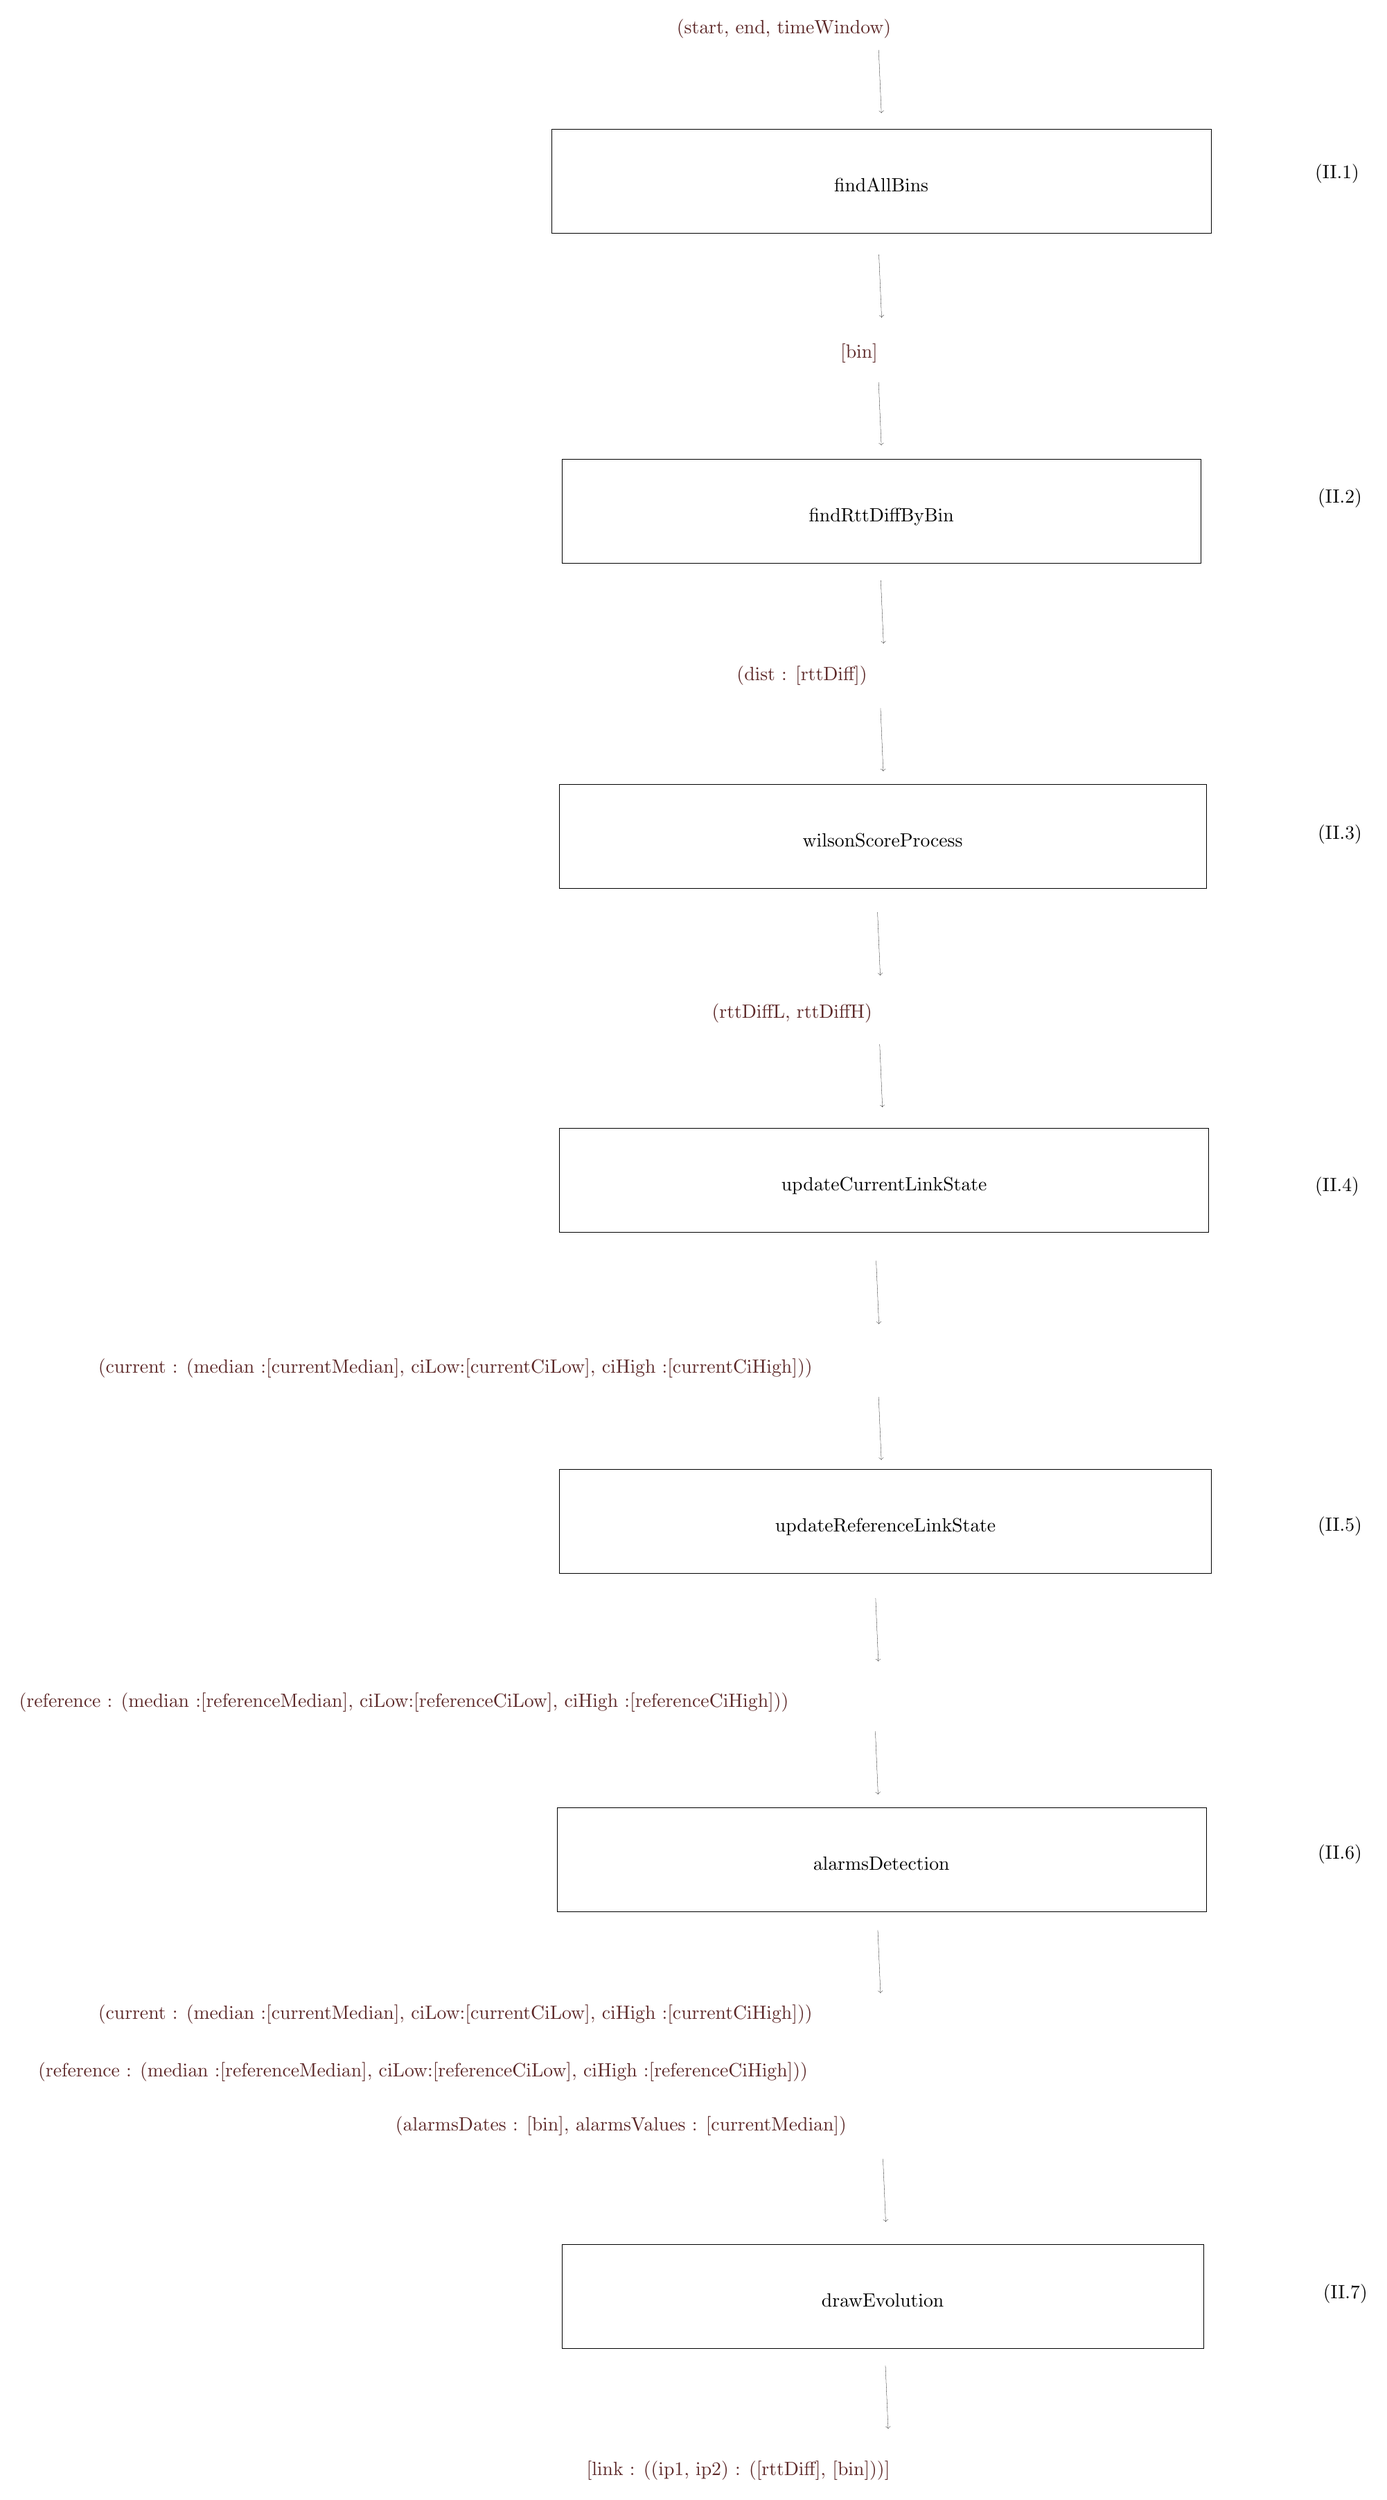
\begin{tikzpicture}[even odd rule]
\pgftransformxscale{1.000000}
\pgftransformyscale{-1.000000}
\definecolor{dialinecolor}{rgb}{0.000000, 0.000000, 0.000000}
\pgfsetstrokecolor{dialinecolor}
\pgfsetstrokeopacity{1.000000}
\definecolor{diafillcolor}{rgb}{1.000000, 1.000000, 1.000000}
\pgfsetfillcolor{diafillcolor}
\pgfsetfillopacity{1.000000}
\pgfsetlinewidth{0.100000\du}
\pgfsetdash{}{0pt}
\pgfsetmiterjoin
{\pgfsetcornersarced{\pgfpoint{0.000000\du}{0.000000\du}}\definecolor{diafillcolor}{rgb}{1.000000, 1.000000, 1.000000}
\pgfsetfillcolor{diafillcolor}
\pgfsetfillopacity{1.000000}
\fill (14.000000\du,7.300000\du)--(14.000000\du,9.200000\du)--(26.100000\du,9.200000\du)--(26.100000\du,7.300000\du)--cycle;
}{\pgfsetcornersarced{\pgfpoint{0.000000\du}{0.000000\du}}\definecolor{dialinecolor}{rgb}{0.000000, 0.000000, 0.000000}
\pgfsetstrokecolor{dialinecolor}
\pgfsetstrokeopacity{1.000000}
\draw (14.000000\du,7.300000\du)--(14.000000\du,9.200000\du)--(26.100000\du,9.200000\du)--(26.100000\du,7.300000\du)--cycle;
}% setfont left to latex
\definecolor{dialinecolor}{rgb}{0.000000, 0.000000, 0.000000}
\pgfsetstrokecolor{dialinecolor}
\pgfsetstrokeopacity{1.000000}
\definecolor{diafillcolor}{rgb}{0.000000, 0.000000, 0.000000}
\pgfsetfillcolor{diafillcolor}
\pgfsetfillopacity{1.000000}
\node[anchor=base,inner sep=0pt, outer sep=0pt,color=dialinecolor] at (20.050000\du,8.445000\du){findAllBins};
% setfont left to latex
\definecolor{dialinecolor}{rgb}{0.360784, 0.152941, 0.152941}
\pgfsetstrokecolor{dialinecolor}
\pgfsetstrokeopacity{1.000000}
\definecolor{diafillcolor}{rgb}{0.360784, 0.152941, 0.152941}
\pgfsetfillcolor{diafillcolor}
\pgfsetfillopacity{1.000000}
\node[anchor=base west,inner sep=0pt,outer sep=0pt,color=dialinecolor] at (16.300000\du,5.550000\du){(start, end, timeWindow)};
\pgfsetlinewidth{0.100000\du}
\pgfsetdash{}{0pt}
\pgfsetbuttcap
{
\definecolor{diafillcolor}{rgb}{0.000000, 0.000000, 0.000000}
\pgfsetfillcolor{diafillcolor}
\pgfsetfillopacity{1.000000}
% was here!!!
\pgfsetarrowsend{to}
\definecolor{dialinecolor}{rgb}{0.000000, 0.000000, 0.000000}
\pgfsetstrokecolor{dialinecolor}
\pgfsetstrokeopacity{1.000000}
\draw (20.000000\du,5.850000\du)--(20.050000\du,7.005000\du);
}
% setfont left to latex
\definecolor{dialinecolor}{rgb}{0.360784, 0.152941, 0.152941}
\pgfsetstrokecolor{dialinecolor}
\pgfsetstrokeopacity{1.000000}
\definecolor{diafillcolor}{rgb}{0.360784, 0.152941, 0.152941}
\pgfsetfillcolor{diafillcolor}
\pgfsetfillopacity{1.000000}
\node[anchor=base west,inner sep=0pt,outer sep=0pt,color=dialinecolor] at (19.300000\du,11.500000\du){\ensuremath{[}bin\ensuremath{]}};
\pgfsetlinewidth{0.100000\du}
\pgfsetdash{}{0pt}
\pgfsetmiterjoin
{\pgfsetcornersarced{\pgfpoint{0.000000\du}{0.000000\du}}\definecolor{diafillcolor}{rgb}{1.000000, 1.000000, 1.000000}
\pgfsetfillcolor{diafillcolor}
\pgfsetfillopacity{1.000000}
\fill (14.200000\du,13.350000\du)--(14.200000\du,15.250000\du)--(25.900000\du,15.250000\du)--(25.900000\du,13.350000\du)--cycle;
}{\pgfsetcornersarced{\pgfpoint{0.000000\du}{0.000000\du}}\definecolor{dialinecolor}{rgb}{0.000000, 0.000000, 0.000000}
\pgfsetstrokecolor{dialinecolor}
\pgfsetstrokeopacity{1.000000}
\draw (14.200000\du,13.350000\du)--(14.200000\du,15.250000\du)--(25.900000\du,15.250000\du)--(25.900000\du,13.350000\du)--cycle;
}% setfont left to latex
\definecolor{dialinecolor}{rgb}{0.000000, 0.000000, 0.000000}
\pgfsetstrokecolor{dialinecolor}
\pgfsetstrokeopacity{1.000000}
\definecolor{diafillcolor}{rgb}{0.000000, 0.000000, 0.000000}
\pgfsetfillcolor{diafillcolor}
\pgfsetfillopacity{1.000000}
\node[anchor=base,inner sep=0pt, outer sep=0pt,color=dialinecolor] at (20.050000\du,14.495000\du){findRttDiffByBin};
% setfont left to latex
\definecolor{dialinecolor}{rgb}{0.360784, 0.152941, 0.152941}
\pgfsetstrokecolor{dialinecolor}
\pgfsetstrokeopacity{1.000000}
\definecolor{diafillcolor}{rgb}{0.360784, 0.152941, 0.152941}
\pgfsetfillcolor{diafillcolor}
\pgfsetfillopacity{1.000000}
\node[anchor=base west,inner sep=0pt,outer sep=0pt,color=dialinecolor] at (17.400000\du,17.400000\du){(dist : \ensuremath{[}rttDiff\ensuremath{]})};
\pgfsetlinewidth{0.100000\du}
\pgfsetdash{}{0pt}
\pgfsetmiterjoin
{\pgfsetcornersarced{\pgfpoint{0.000000\du}{0.000000\du}}\definecolor{diafillcolor}{rgb}{1.000000, 1.000000, 1.000000}
\pgfsetfillcolor{diafillcolor}
\pgfsetfillopacity{1.000000}
\fill (14.150000\du,19.300000\du)--(14.150000\du,21.200000\du)--(26.000000\du,21.200000\du)--(26.000000\du,19.300000\du)--cycle;
}{\pgfsetcornersarced{\pgfpoint{0.000000\du}{0.000000\du}}\definecolor{dialinecolor}{rgb}{0.000000, 0.000000, 0.000000}
\pgfsetstrokecolor{dialinecolor}
\pgfsetstrokeopacity{1.000000}
\draw (14.150000\du,19.300000\du)--(14.150000\du,21.200000\du)--(26.000000\du,21.200000\du)--(26.000000\du,19.300000\du)--cycle;
}% setfont left to latex
\definecolor{dialinecolor}{rgb}{0.000000, 0.000000, 0.000000}
\pgfsetstrokecolor{dialinecolor}
\pgfsetstrokeopacity{1.000000}
\definecolor{diafillcolor}{rgb}{0.000000, 0.000000, 0.000000}
\pgfsetfillcolor{diafillcolor}
\pgfsetfillopacity{1.000000}
\node[anchor=base,inner sep=0pt, outer sep=0pt,color=dialinecolor] at (20.075000\du,20.445000\du){wilsonScoreProcess};
% setfont left to latex
\definecolor{dialinecolor}{rgb}{0.360784, 0.152941, 0.152941}
\pgfsetstrokecolor{dialinecolor}
\pgfsetstrokeopacity{1.000000}
\definecolor{diafillcolor}{rgb}{0.360784, 0.152941, 0.152941}
\pgfsetfillcolor{diafillcolor}
\pgfsetfillopacity{1.000000}
\node[anchor=base west,inner sep=0pt,outer sep=0pt,color=dialinecolor] at (16.945000\du,23.585000\du){(rttDiffL, rttDiffH)};
\pgfsetlinewidth{0.100000\du}
\pgfsetdash{}{0pt}
\pgfsetmiterjoin
{\pgfsetcornersarced{\pgfpoint{0.000000\du}{0.000000\du}}\definecolor{diafillcolor}{rgb}{1.000000, 1.000000, 1.000000}
\pgfsetfillcolor{diafillcolor}
\pgfsetfillopacity{1.000000}
\fill (14.150000\du,25.600000\du)--(14.150000\du,27.500000\du)--(26.050000\du,27.500000\du)--(26.050000\du,25.600000\du)--cycle;
}{\pgfsetcornersarced{\pgfpoint{0.000000\du}{0.000000\du}}\definecolor{dialinecolor}{rgb}{0.000000, 0.000000, 0.000000}
\pgfsetstrokecolor{dialinecolor}
\pgfsetstrokeopacity{1.000000}
\draw (14.150000\du,25.600000\du)--(14.150000\du,27.500000\du)--(26.050000\du,27.500000\du)--(26.050000\du,25.600000\du)--cycle;
}% setfont left to latex
\definecolor{dialinecolor}{rgb}{0.000000, 0.000000, 0.000000}
\pgfsetstrokecolor{dialinecolor}
\pgfsetstrokeopacity{1.000000}
\definecolor{diafillcolor}{rgb}{0.000000, 0.000000, 0.000000}
\pgfsetfillcolor{diafillcolor}
\pgfsetfillopacity{1.000000}
\node[anchor=base,inner sep=0pt, outer sep=0pt,color=dialinecolor] at (20.100000\du,26.745000\du){updateCurrentLinkState};
% setfont left to latex
\definecolor{dialinecolor}{rgb}{0.360784, 0.152941, 0.152941}
\pgfsetstrokecolor{dialinecolor}
\pgfsetstrokeopacity{1.000000}
\definecolor{diafillcolor}{rgb}{0.360784, 0.152941, 0.152941}
\pgfsetfillcolor{diafillcolor}
\pgfsetfillopacity{1.000000}
\node[anchor=base west,inner sep=0pt,outer sep=0pt,color=dialinecolor] at (5.695000\du,30.085000\du){(current : (median :\ensuremath{[}currentMedian\ensuremath{]}, ciLow:\ensuremath{[}currentCiLow\ensuremath{]}, ciHigh :\ensuremath{[}currentCiHigh\ensuremath{]}))};
\pgfsetlinewidth{0.100000\du}
\pgfsetdash{}{0pt}
\pgfsetmiterjoin
{\pgfsetcornersarced{\pgfpoint{0.000000\du}{0.000000\du}}\definecolor{diafillcolor}{rgb}{1.000000, 1.000000, 1.000000}
\pgfsetfillcolor{diafillcolor}
\pgfsetfillopacity{1.000000}
\fill (14.150000\du,31.850000\du)--(14.150000\du,33.750000\du)--(26.100000\du,33.750000\du)--(26.100000\du,31.850000\du)--cycle;
}{\pgfsetcornersarced{\pgfpoint{0.000000\du}{0.000000\du}}\definecolor{dialinecolor}{rgb}{0.000000, 0.000000, 0.000000}
\pgfsetstrokecolor{dialinecolor}
\pgfsetstrokeopacity{1.000000}
\draw (14.150000\du,31.850000\du)--(14.150000\du,33.750000\du)--(26.100000\du,33.750000\du)--(26.100000\du,31.850000\du)--cycle;
}% setfont left to latex
\definecolor{dialinecolor}{rgb}{0.000000, 0.000000, 0.000000}
\pgfsetstrokecolor{dialinecolor}
\pgfsetstrokeopacity{1.000000}
\definecolor{diafillcolor}{rgb}{0.000000, 0.000000, 0.000000}
\pgfsetfillcolor{diafillcolor}
\pgfsetfillopacity{1.000000}
\node[anchor=base,inner sep=0pt, outer sep=0pt,color=dialinecolor] at (20.125000\du,32.995000\du){updateReferenceLinkState};
\pgfsetlinewidth{0.100000\du}
\pgfsetdash{}{0pt}
\pgfsetmiterjoin
{\pgfsetcornersarced{\pgfpoint{0.000000\du}{0.000000\du}}\definecolor{diafillcolor}{rgb}{1.000000, 1.000000, 1.000000}
\pgfsetfillcolor{diafillcolor}
\pgfsetfillopacity{1.000000}
\fill (14.100000\du,38.050000\du)--(14.100000\du,39.950000\du)--(26.000000\du,39.950000\du)--(26.000000\du,38.050000\du)--cycle;
}{\pgfsetcornersarced{\pgfpoint{0.000000\du}{0.000000\du}}\definecolor{dialinecolor}{rgb}{0.000000, 0.000000, 0.000000}
\pgfsetstrokecolor{dialinecolor}
\pgfsetstrokeopacity{1.000000}
\draw (14.100000\du,38.050000\du)--(14.100000\du,39.950000\du)--(26.000000\du,39.950000\du)--(26.000000\du,38.050000\du)--cycle;
}% setfont left to latex
\definecolor{dialinecolor}{rgb}{0.000000, 0.000000, 0.000000}
\pgfsetstrokecolor{dialinecolor}
\pgfsetstrokeopacity{1.000000}
\definecolor{diafillcolor}{rgb}{0.000000, 0.000000, 0.000000}
\pgfsetfillcolor{diafillcolor}
\pgfsetfillopacity{1.000000}
\node[anchor=base,inner sep=0pt, outer sep=0pt,color=dialinecolor] at (20.050000\du,39.195000\du){alarmsDetection};
\pgfsetlinewidth{0.100000\du}
\pgfsetdash{}{0pt}
\pgfsetmiterjoin
{\pgfsetcornersarced{\pgfpoint{0.000000\du}{0.000000\du}}\definecolor{diafillcolor}{rgb}{1.000000, 1.000000, 1.000000}
\pgfsetfillcolor{diafillcolor}
\pgfsetfillopacity{1.000000}
\fill (14.200000\du,46.050000\du)--(14.200000\du,47.950000\du)--(25.950000\du,47.950000\du)--(25.950000\du,46.050000\du)--cycle;
}{\pgfsetcornersarced{\pgfpoint{0.000000\du}{0.000000\du}}\definecolor{dialinecolor}{rgb}{0.000000, 0.000000, 0.000000}
\pgfsetstrokecolor{dialinecolor}
\pgfsetstrokeopacity{1.000000}
\draw (14.200000\du,46.050000\du)--(14.200000\du,47.950000\du)--(25.950000\du,47.950000\du)--(25.950000\du,46.050000\du)--cycle;
}% setfont left to latex
\definecolor{dialinecolor}{rgb}{0.000000, 0.000000, 0.000000}
\pgfsetstrokecolor{dialinecolor}
\pgfsetstrokeopacity{1.000000}
\definecolor{diafillcolor}{rgb}{0.000000, 0.000000, 0.000000}
\pgfsetfillcolor{diafillcolor}
\pgfsetfillopacity{1.000000}
\node[anchor=base,inner sep=0pt, outer sep=0pt,color=dialinecolor] at (20.075000\du,47.195000\du){drawEvolution};
% setfont left to latex
\definecolor{dialinecolor}{rgb}{0.360784, 0.152941, 0.152941}
\pgfsetstrokecolor{dialinecolor}
\pgfsetstrokeopacity{1.000000}
\definecolor{diafillcolor}{rgb}{0.360784, 0.152941, 0.152941}
\pgfsetfillcolor{diafillcolor}
\pgfsetfillopacity{1.000000}
\node[anchor=base west,inner sep=0pt,outer sep=0pt,color=dialinecolor] at (14.645000\du,50.285000\du){\ensuremath{[}link : ((ip1, ip2) : (\ensuremath{[}rttDiff\ensuremath{]}, \ensuremath{[}bin\ensuremath{]}))\ensuremath{]}};
\pgfsetlinewidth{0.100000\du}
\pgfsetdash{}{0pt}
\pgfsetbuttcap
{
\definecolor{diafillcolor}{rgb}{0.000000, 0.000000, 0.000000}
\pgfsetfillcolor{diafillcolor}
\pgfsetfillopacity{1.000000}
% was here!!!
\pgfsetarrowsend{to}
\definecolor{dialinecolor}{rgb}{0.000000, 0.000000, 0.000000}
\pgfsetstrokecolor{dialinecolor}
\pgfsetstrokeopacity{1.000000}
\draw (20.004200\du,9.597120\du)--(20.054200\du,10.752100\du);
}
\pgfsetlinewidth{0.100000\du}
\pgfsetdash{}{0pt}
\pgfsetbuttcap
{
\definecolor{diafillcolor}{rgb}{0.000000, 0.000000, 0.000000}
\pgfsetfillcolor{diafillcolor}
\pgfsetfillopacity{1.000000}
% was here!!!
\pgfsetarrowsend{to}
\definecolor{dialinecolor}{rgb}{0.000000, 0.000000, 0.000000}
\pgfsetstrokecolor{dialinecolor}
\pgfsetstrokeopacity{1.000000}
\draw (19.999200\du,11.937100\du)--(20.049200\du,13.092100\du);
}
\pgfsetlinewidth{0.100000\du}
\pgfsetdash{}{0pt}
\pgfsetbuttcap
{
\definecolor{diafillcolor}{rgb}{0.000000, 0.000000, 0.000000}
\pgfsetfillcolor{diafillcolor}
\pgfsetfillopacity{1.000000}
% was here!!!
\pgfsetarrowsend{to}
\definecolor{dialinecolor}{rgb}{0.000000, 0.000000, 0.000000}
\pgfsetstrokecolor{dialinecolor}
\pgfsetstrokeopacity{1.000000}
\draw (20.039200\du,15.567100\du)--(20.089200\du,16.722100\du);
}
\pgfsetlinewidth{0.100000\du}
\pgfsetdash{}{0pt}
\pgfsetbuttcap
{
\definecolor{diafillcolor}{rgb}{0.000000, 0.000000, 0.000000}
\pgfsetfillcolor{diafillcolor}
\pgfsetfillopacity{1.000000}
% was here!!!
\pgfsetarrowsend{to}
\definecolor{dialinecolor}{rgb}{0.000000, 0.000000, 0.000000}
\pgfsetstrokecolor{dialinecolor}
\pgfsetstrokeopacity{1.000000}
\draw (20.034200\du,17.907100\du)--(20.084200\du,19.062100\du);
}
\pgfsetlinewidth{0.100000\du}
\pgfsetdash{}{0pt}
\pgfsetbuttcap
{
\definecolor{diafillcolor}{rgb}{0.000000, 0.000000, 0.000000}
\pgfsetfillcolor{diafillcolor}
\pgfsetfillopacity{1.000000}
% was here!!!
\pgfsetarrowsend{to}
\definecolor{dialinecolor}{rgb}{0.000000, 0.000000, 0.000000}
\pgfsetstrokecolor{dialinecolor}
\pgfsetstrokeopacity{1.000000}
\draw (19.979200\du,21.647100\du)--(20.029200\du,22.802100\du);
}
\pgfsetlinewidth{0.100000\du}
\pgfsetdash{}{0pt}
\pgfsetbuttcap
{
\definecolor{diafillcolor}{rgb}{0.000000, 0.000000, 0.000000}
\pgfsetfillcolor{diafillcolor}
\pgfsetfillopacity{1.000000}
% was here!!!
\pgfsetarrowsend{to}
\definecolor{dialinecolor}{rgb}{0.000000, 0.000000, 0.000000}
\pgfsetstrokecolor{dialinecolor}
\pgfsetstrokeopacity{1.000000}
\draw (20.019200\du,24.062700\du)--(20.069200\du,25.217700\du);
}
\pgfsetlinewidth{0.100000\du}
\pgfsetdash{}{0pt}
\pgfsetbuttcap
{
\definecolor{diafillcolor}{rgb}{0.000000, 0.000000, 0.000000}
\pgfsetfillcolor{diafillcolor}
\pgfsetfillopacity{1.000000}
% was here!!!
\pgfsetarrowsend{to}
\definecolor{dialinecolor}{rgb}{0.000000, 0.000000, 0.000000}
\pgfsetstrokecolor{dialinecolor}
\pgfsetstrokeopacity{1.000000}
\draw (19.954200\du,28.032700\du)--(20.004200\du,29.187700\du);
}
\pgfsetlinewidth{0.100000\du}
\pgfsetdash{}{0pt}
\pgfsetbuttcap
{
\definecolor{diafillcolor}{rgb}{0.000000, 0.000000, 0.000000}
\pgfsetfillcolor{diafillcolor}
\pgfsetfillopacity{1.000000}
% was here!!!
\pgfsetarrowsend{to}
\definecolor{dialinecolor}{rgb}{0.000000, 0.000000, 0.000000}
\pgfsetstrokecolor{dialinecolor}
\pgfsetstrokeopacity{1.000000}
\draw (19.999200\du,30.522700\du)--(20.049200\du,31.677700\du);
}
\pgfsetlinewidth{0.100000\du}
\pgfsetdash{}{0pt}
\pgfsetbuttcap
{
\definecolor{diafillcolor}{rgb}{0.000000, 0.000000, 0.000000}
\pgfsetfillcolor{diafillcolor}
\pgfsetfillopacity{1.000000}
% was here!!!
\pgfsetarrowsend{to}
\definecolor{dialinecolor}{rgb}{0.000000, 0.000000, 0.000000}
\pgfsetstrokecolor{dialinecolor}
\pgfsetstrokeopacity{1.000000}
\draw (19.944200\du,34.212700\du)--(19.994200\du,35.367700\du);
}
\pgfsetlinewidth{0.100000\du}
\pgfsetdash{}{0pt}
\pgfsetbuttcap
{
\definecolor{diafillcolor}{rgb}{0.000000, 0.000000, 0.000000}
\pgfsetfillcolor{diafillcolor}
\pgfsetfillopacity{1.000000}
% was here!!!
\pgfsetarrowsend{to}
\definecolor{dialinecolor}{rgb}{0.000000, 0.000000, 0.000000}
\pgfsetstrokecolor{dialinecolor}
\pgfsetstrokeopacity{1.000000}
\draw (19.939200\du,36.649600\du)--(19.989200\du,37.804600\du);
}
\pgfsetlinewidth{0.100000\du}
\pgfsetdash{}{0pt}
\pgfsetbuttcap
{
\definecolor{diafillcolor}{rgb}{0.000000, 0.000000, 0.000000}
\pgfsetfillcolor{diafillcolor}
\pgfsetfillopacity{1.000000}
% was here!!!
\pgfsetarrowsend{to}
\definecolor{dialinecolor}{rgb}{0.000000, 0.000000, 0.000000}
\pgfsetstrokecolor{dialinecolor}
\pgfsetstrokeopacity{1.000000}
\draw (19.984200\du,40.289600\du)--(20.034200\du,41.444600\du);
}
\pgfsetlinewidth{0.100000\du}
\pgfsetdash{}{0pt}
\pgfsetbuttcap
{
\definecolor{diafillcolor}{rgb}{0.000000, 0.000000, 0.000000}
\pgfsetfillcolor{diafillcolor}
\pgfsetfillopacity{1.000000}
% was here!!!
\pgfsetarrowsend{to}
\definecolor{dialinecolor}{rgb}{0.000000, 0.000000, 0.000000}
\pgfsetstrokecolor{dialinecolor}
\pgfsetstrokeopacity{1.000000}
\draw (20.079200\du,44.479600\du)--(20.129200\du,45.634600\du);
}
\pgfsetlinewidth{0.100000\du}
\pgfsetdash{}{0pt}
\pgfsetbuttcap
{
\definecolor{diafillcolor}{rgb}{0.000000, 0.000000, 0.000000}
\pgfsetfillcolor{diafillcolor}
\pgfsetfillopacity{1.000000}
% was here!!!
\pgfsetarrowsend{to}
\definecolor{dialinecolor}{rgb}{0.000000, 0.000000, 0.000000}
\pgfsetstrokecolor{dialinecolor}
\pgfsetstrokeopacity{1.000000}
\draw (20.124200\du,48.269600\du)--(20.174200\du,49.424600\du);
}
% setfont left to latex
\definecolor{dialinecolor}{rgb}{0.000000, 0.000000, 0.000000}
\pgfsetstrokecolor{dialinecolor}
\pgfsetstrokeopacity{1.000000}
\definecolor{diafillcolor}{rgb}{0.000000, 0.000000, 0.000000}
\pgfsetfillcolor{diafillcolor}
\pgfsetfillopacity{1.000000}
\node[anchor=base west,inner sep=0pt,outer sep=0pt,color=dialinecolor] at (28.000000\du,8.205000\du){(II.1)};
% setfont left to latex
\definecolor{dialinecolor}{rgb}{0.000000, 0.000000, 0.000000}
\pgfsetstrokecolor{dialinecolor}
\pgfsetstrokeopacity{1.000000}
\definecolor{diafillcolor}{rgb}{0.000000, 0.000000, 0.000000}
\pgfsetfillcolor{diafillcolor}
\pgfsetfillopacity{1.000000}
\node[anchor=base west,inner sep=0pt,outer sep=0pt,color=dialinecolor] at (28.050000\du,14.155000\du){(II.2)};
% setfont left to latex
\definecolor{dialinecolor}{rgb}{0.000000, 0.000000, 0.000000}
\pgfsetstrokecolor{dialinecolor}
\pgfsetstrokeopacity{1.000000}
\definecolor{diafillcolor}{rgb}{0.000000, 0.000000, 0.000000}
\pgfsetfillcolor{diafillcolor}
\pgfsetfillopacity{1.000000}
\node[anchor=base west,inner sep=0pt,outer sep=0pt,color=dialinecolor] at (28.050000\du,20.305000\du){(II.3)};
% setfont left to latex
\definecolor{dialinecolor}{rgb}{0.000000, 0.000000, 0.000000}
\pgfsetstrokecolor{dialinecolor}
\pgfsetstrokeopacity{1.000000}
\definecolor{diafillcolor}{rgb}{0.000000, 0.000000, 0.000000}
\pgfsetfillcolor{diafillcolor}
\pgfsetfillopacity{1.000000}
\node[anchor=base west,inner sep=0pt,outer sep=0pt,color=dialinecolor] at (28.000000\du,26.755000\du){(II.4)};
% setfont left to latex
\definecolor{dialinecolor}{rgb}{0.000000, 0.000000, 0.000000}
\pgfsetstrokecolor{dialinecolor}
\pgfsetstrokeopacity{1.000000}
\definecolor{diafillcolor}{rgb}{0.000000, 0.000000, 0.000000}
\pgfsetfillcolor{diafillcolor}
\pgfsetfillopacity{1.000000}
\node[anchor=base west,inner sep=0pt,outer sep=0pt,color=dialinecolor] at (28.050000\du,32.987500\du){(II.5)};
% setfont left to latex
\definecolor{dialinecolor}{rgb}{0.000000, 0.000000, 0.000000}
\pgfsetstrokecolor{dialinecolor}
\pgfsetstrokeopacity{1.000000}
\definecolor{diafillcolor}{rgb}{0.000000, 0.000000, 0.000000}
\pgfsetfillcolor{diafillcolor}
\pgfsetfillopacity{1.000000}
\node[anchor=base west,inner sep=0pt,outer sep=0pt,color=dialinecolor] at (28.050000\du,38.987500\du){(II.6)};
% setfont left to latex
\definecolor{dialinecolor}{rgb}{0.000000, 0.000000, 0.000000}
\pgfsetstrokecolor{dialinecolor}
\pgfsetstrokeopacity{1.000000}
\definecolor{diafillcolor}{rgb}{0.000000, 0.000000, 0.000000}
\pgfsetfillcolor{diafillcolor}
\pgfsetfillopacity{1.000000}
\node[anchor=base west,inner sep=0pt,outer sep=0pt,color=dialinecolor] at (28.150000\du,47.037500\du){(II.7)};
% setfont left to latex
\definecolor{dialinecolor}{rgb}{0.360784, 0.152941, 0.152941}
\pgfsetstrokecolor{dialinecolor}
\pgfsetstrokeopacity{1.000000}
\definecolor{diafillcolor}{rgb}{0.360784, 0.152941, 0.152941}
\pgfsetfillcolor{diafillcolor}
\pgfsetfillopacity{1.000000}
\node[anchor=base west,inner sep=0pt,outer sep=0pt,color=dialinecolor] at (4.245000\du,36.207900\du){(reference : (median :\ensuremath{[}referenceMedian\ensuremath{]}, ciLow:\ensuremath{[}referenceCiLow\ensuremath{]}, ciHigh :\ensuremath{[}referenceCiHigh\ensuremath{]}))};
% setfont left to latex
\definecolor{dialinecolor}{rgb}{0.360784, 0.152941, 0.152941}
\pgfsetstrokecolor{dialinecolor}
\pgfsetstrokeopacity{1.000000}
\definecolor{diafillcolor}{rgb}{0.360784, 0.152941, 0.152941}
\pgfsetfillcolor{diafillcolor}
\pgfsetfillopacity{1.000000}
\node[anchor=base west,inner sep=0pt,outer sep=0pt,color=dialinecolor] at (5.695000\du,41.922500\du){(current : (median :\ensuremath{[}currentMedian\ensuremath{]}, ciLow:\ensuremath{[}currentCiLow\ensuremath{]}, ciHigh :\ensuremath{[}currentCiHigh\ensuremath{]}))};
% setfont left to latex
\definecolor{dialinecolor}{rgb}{0.360784, 0.152941, 0.152941}
\pgfsetstrokecolor{dialinecolor}
\pgfsetstrokeopacity{1.000000}
\definecolor{diafillcolor}{rgb}{0.360784, 0.152941, 0.152941}
\pgfsetfillcolor{diafillcolor}
\pgfsetfillopacity{1.000000}
\node[anchor=base west,inner sep=0pt,outer sep=0pt,color=dialinecolor] at (4.595000\du,42.972500\du){(reference : (median :\ensuremath{[}referenceMedian\ensuremath{]}, ciLow:\ensuremath{[}referenceCiLow\ensuremath{]}, ciHigh :\ensuremath{[}referenceCiHigh\ensuremath{]}))};
% setfont left to latex
\definecolor{dialinecolor}{rgb}{0.360784, 0.152941, 0.152941}
\pgfsetstrokecolor{dialinecolor}
\pgfsetstrokeopacity{1.000000}
\definecolor{diafillcolor}{rgb}{0.360784, 0.152941, 0.152941}
\pgfsetfillcolor{diafillcolor}
\pgfsetfillopacity{1.000000}
\node[anchor=base west,inner sep=0pt,outer sep=0pt,color=dialinecolor] at (11.145000\du,43.972500\du){(alarmsDates : \ensuremath{[}bin\ensuremath{]}, alarmsValues : \ensuremath{[}currentMedian\ensuremath{]})};
\end{tikzpicture}

	}
	\caption{Phase II : détection des changements }
	\label{fig:step-detection-anomalies}
\end{figure}

\subsection{Exemple illustratif }

\paragraph{Description de  l'échantillon} :

L'échantillon des traceroutes qui va nous permettre d'illustrer l'algorithme de la détection est définit comme suit :

\begin{itemize}
	\item le nombre total des traceroutes est de $24$;
	\item le premier traceroute a été capturé à $1514769800$ (GMT: Monday, January 1, 2018 1:23:20);
	\item le dernier traceroute capturé à $1514787809$ (GMT: Monday, January 1, 2018 6:23:29 );
	\item la durée d'une période est $1$ heure ($3600$);
	\item les débuts des périodes entre $ 1514769800 $ et $ 1514789809 $ sont  $ 1514769800 $, $ 1514773400 $, $ 1514777000 $, $ 1514780600 $, $ 1514784200 $, $ 1514787800 $;
	\item la liste des traceroutes analysés est disponible sur[!].
\end{itemize} 



%\begin{landscape}

\begin{table}[H]
	\centering
	%\resizebox{\textwidth}{!}{
	\begin{tabularx}{\linewidth}{|c|c|}
	étape &  outputs	\\ \hline
	(I.1) &   $ 1514769800 $, $ 1514773400 $, $ 1514777000 $,
	
	 $ 1514780600 $, $ 1514784200 $, $ 1514787800 $\\ \hline
(I.2)& 
				\begin{tabular}{ccc}
	Id&	Période& nombre de traceroutes \\ \hline
	1&	[1514769800, 1514769800+3600] & 4\\ \hline
	2&	[1514773400, 1514773400+3600] & 4\\ \hline
	3&	[1514777000, 1514777000+3600] & 4\\ \hline
	4&	[1514780600, 1514780600+3600] &4 \\ \hline
	5&	[1514784200, 1514784200+3600] &4 \\ \hline
	6&	[1514787800, 1514787800+3600] & 4 \\ \hline
				\end{tabular}\\ \hline
\end{tabularx}
%}
\end{table}

Une fois les traceroutes sont groupés par période, nous parcourons chaque traceroute afin d'éliminer ceux invalides (removeInvalidTraceroute I.3). 

Ensuite, nous agrégeons chaque saut par source de signal en calculant leur médiane. Nous donnons un exemple d'un traceroute qui illustre cette agrégation. Le même traitement est appliqué sur tout traceroute. 

\begin{lstlisting}[language=json,firstnumber=1, caption={Les saut du traceroute T7 (sans agrégation)}]
hop_id : 1, hops : [(from : 89.105.200.57, rtt : 1.955,  x : None),(from : 89.105.200.57, rtt : 1.7, x : None),(from : 89.105.200.57, rtt : 1.709,  x : None)]
hop_id : 2, hops : [(from : 185.147.12.31, rtt : 8.543,  x : None),(from : 185.147.12.31, rtt : 4.103, x : None),(from : 185.147.12.31, rtt : 4.41, x : None)]
hop_id : 3, hops : [(from : 185.147.12.19, rtt : 4.347,  x : None),(from : 185.147.12.19, rtt : 2.876, x : None),(from : 185.147.12.19, rtt : 3.143, x : None )]
\end{lstlisting}

\begin{lstlisting}[language=json,firstnumber=1, caption={Les saut du traceroute T7 (après l'agrégation)}]
hop_id : 1, hops : [(from : 89.105.200.57, rttAgg : 1.709)]
hop_id : 2, hops : [(from : 185.147.12.31, rttAgg : 4.41)] 
hop_id : 3, hops : [(from : 185.147.12.19, rttAgg : 3.143)]
\end{lstlisting}

L'inférence (I.5) des liens du traceroute T7 donne les liens suivants: 

\begin{lstlisting}[language=json,firstnumber=1, caption={Exemple des liens inférés du traceroute T7}, basicstyle = \small]
lien 1 : (link : (185.147.12.31, 89.105.200.57), rttDiff : 2.701)
lien 2 : (link : (185.147.12.19,185.147.12.31), rttDiff : -1.267)
\end{lstlisting}


A l'étape (I.6), nous ordonnons chaque lien, nous ordonnons plutôt leurs adresses IP comme illustré ci-dessous avec la fonction \textit{sort()}. 

\begin{lstlisting}[language=json,firstnumber=1, caption={Illustration de l'ordre des liens}, basicstyle = \footnotesize]
sort(("185.147.12.31","89.105.200.57")) = ("185.147.12.31","89.105.200.57")
sort(("89.105.200.57","185.147.12.31"))= ("185.147.12.31","89.105.200.57")   
\end{lstlisting}

L'ordonnancement à l'étape  (I.6) est une préparation à la fusion. Nous fusionnons les liens ayant impliqué les mêmes routeurs dans une même période. Prenons les liens inférés à partir de $5$ traceroutes  comme c'est montré ci-dessous :

\begin{lstlisting}[language=json,firstnumber=1, caption={Liste des liens possibles inférés via  les traceroutes T1, T2, T3, T4 et T5}, basicstyle = \footnotesize]
T1 (link : (185.147.12.31,89.105.200.57), rttDiff : 2.463)
   (link : (185.147.12.19,185.147.12.31), rttDiff : -1.029)

T2 (link : (185.147.12.31,89.105.200.57), rttDiff : 3.463) 
   (link : (185.147.12.19,185.147.12.31), rttDiff : -2.029)

T3 (link : (185.147.12.31,89.105.200.57), rttDiff : 2.991) 
   (link : (185.147.12.19,185.147.12.31), rttDiff : -1.557)

T4 (link : (185.147.12.31,89.105.200.57), rttDiff : 4.631) 
   (link : (185.147.12.19,185.147.12.31), rttDiff : -3.197)

T5 (link : (89.105.200.57,185.147.12.31), rttDiff : -7.75) 
   (link : (185.147.12.19,89.105.200.57), rttDiff : 3.803)
\end{lstlisting}

La fusion de ces liens nous donne les trois liens ci-dessous. Chaque lien est caractérisé par les sondes l'ayant capturé, leurs  RTTs Différentiels et la période dupliquée, pendant laquelle il a été identifié, en nombre de RTT différentiel. 

\begin{lstlisting}[language=json,firstnumber=1, caption={Caractérisation des liens identifiés lors  de la période 1514769800 avec les traceroutes T1, T2, T3, T4 et T5}, basicstyle = \footnotesize, ]
[(link :(185.147.12.19,89.105.200.57),
probes : [4247],
rttDiffs :[3.803],
bins :[1514769800]),

(link : (185.147.12.19,185.147.12.31),
probes : [4247, 4247, 4247, 4247],
rttDiffs :[-1.029, -2.029, -1.557, -3.197],
bins : [1514769800, 1514769800, 1514769800, 1514769800]),

(link : (185.147.12.31,89.105.200.57),
probes : [4247, 4247, 4247, 4247, 4247],
rttDiffs :[2.463, 3.463, 2.991, 4.631, -7.75],
bins : [1514769800, 1514769800, 1514769800, 1514769800, 1514769800]) ]
\end{lstlisting}

Après avoir analysé  toutes les périodes, nous résumons les liens en fusionnant les données relatives à toutes les périodes, c'est l'objectif de l'étape (I.8).

\begin{lstlisting}[language=json,firstnumber=1, caption={Illustration de l'ordre des liens}, basicstyle = \footnotesize]
[(link   : (185.147.12.19,89.105.200.57), 
    probes : (4247), 
    rttDiffs : (3.803), 
    bins : (1514769800)),  

 link : (185.147.12.19,185.147.12.31), 
    probes : (4247, 4247, 4247, 4247, 4247, 4247, 4247, 4247, 4247, 4247, 4247, 4247, 4247, 4247, 4247, 4247, 4247, 4247, 4247, 4247, 4247, 4247, 4247, 4247), 
    rttDiffs : (-1.267, -2.407, -1.49, -3.029, -1060.029, -1045.029, -1098.029, -1080.029, -680.029, -845.029, -998.029, -800.029, -1.029, -2.029, -1.557, -3.197, -1.277, -2.017, -1.257, -2.968, -0.96, -1.967, -0.987, -3.201), 
    bins : (1514787800, 1514787800, 1514787800, 1514787800, 1514784200, 1514784200, 1514784200, 1514784200, 1514780600, 1514780600, 1514780600, 1514780600, 1514769800, 1514769800, 1514769800, 1514769800, 1514773400, 1514773400, 1514773400, 1514773400, 1514777000, 1514777000, 1514777000, 1514777000)),  

 link : (185.147.12.31,89.105.200.57),
    probes : (4247, 4247, 4247, 4247, 4247, 4247, 4247, 4247, 4247, 4247, 4247, 4247, 4247, 4247, 4247, 4247, 4247, 4247, 4247, 4247, 4247, 4247, 4247, 4247, 4247),
    rttDiffs : (2.701, 3.841, 2.924, 4.463, 1061.463, 1046.463, 1099.463, 1081.463, 681.463, 846.463, 999.463, 801.463, 2.463, 3.463, 2.991, 4.631, -7.75, 2.711, 3.451, 2.691, 4.402, 2.394, 3.401, 2.421, 4.635),
    bins : (1514787800, 1514787800, 1514787800, 1514787800, 1514784200, 1514784200, 1514784200, 1514784200, 1514780600, 1514780600, 1514780600, 1514780600, 1514769800, 1514769800, 1514769800, 1514769800, 1514769800, 1514773400, 1514773400, 1514773400, 1514773400, 1514777000, 1514777000, 1514777000, 1514777000))]
\end{lstlisting}


A la fin de l'étape (I.8), nous disposons de tous les liens possibles caractérisés avec leurs RTTs différentiels. Ainsi, nous pouvons entamer la phase II du processus de la détection.

Dans un premier temps, nous générons les même  périodes générées à  l'étape (I.1). Pour chaque bin,  nous récupérons les RTTs différentiels identifiés durant ce bin, ainsi nous obtenons {\color{gray} dist}, cette dernière représente l'ensemble des RTTs différentiels du bin courant, c'est l'objectif de l'étape (II.2).

Dans notre exemple,  et pour la clarté de ce dernier, une référence est assez représentable après avoir calculé 3 intervalles de confiances. 
\newpage
%\begin{landscape}
	\begin{table}[H]
		\centering

	%	\resizebox{24.7cm}{!}{
		\begin{tabularx}{\linewidth}{|l|X| }
		\hline
itération & 1	\\ \hline
bin & $1514769800$ \\ \hline
lien & $(185.147.12.31, 89.105.200.57)$  \\ \hline
dist& [-7.75, 2.463, 2.991, 3.463, 4.631]	\\ \hline
(low, hight)& (0.11762077423264793, 0.7692757187239873) 	\\ \hline
(lo, hi)&(0.5881038711632396, 3.8463785936199364)  \\ \hline
(l, h) & (0, 3) 	\\ \hline
rttDiffL& dist[0] = -7.75	\\ \hline
rttDiffH& dist[3]= 3.463	\\ \hline
currentMedian& 2.991	\\ \hline
currentCiLow&  2.991 - (-7.75) = 10.741 	\\ \hline
currentCiHi& 3.463 - 2.991 =  0.472	\\ \hline
cas 1? 2? 3?& cas 1 (aucun intervalle de confiance calculé)  \\ \hline
referenceMedian& 2.991	\\ \hline
referenceCiLow& -7.75	\\ \hline
referenceCiHi&3.463	\\ \hline
détection des alarmes ?& non (car cas 3 pas  encore atteint)	\\ \hline
alarmesDates& []	\\ \hline
alarmesValues& []	\\ \hline
		
			
		\end{tabularx}
	%	}
	\end{table}


	\begin{table}[H]
	\centering
	
	%	\resizebox{24.7cm}{!}{
	\begin{tabularx}{\linewidth}{|l|X| }
		\hline
		itération & 2	\\ \hline
		bin & $1514773400$ \\ \hline
		lien & $(185.147.12.31, 89.105.200.57)$  \\ \hline
		dist& [2.691, 2.711, 3.451, 4.402]	\\ \hline
		(low, hight)& (0.15003898915214947, 0.8499610108478506) 	\\ \hline
		(lo, hi)&(0.6001559566085979, 3.3998440433914023)  \\ \hline
		(l, h) & (0, 3) 	\\ \hline
		rttDiffL& dist[0] = 2.691	\\ \hline
		rttDiffH& dist[3]= 4.402	\\ \hline
		currentMedian& 3.081	\\ \hline
		currentCiLow&  0.39 	\\ \hline
		currentCiHi& 1.321	\\ \hline
		cas 1? 2? 3?& cas 1 (1 intervalle de confiance calculé)  \\ \hline
		referenceMedian& 3.081	\\ \hline
		referenceCiLow& 2.691	\\ \hline
		referenceCiHi&4.402	\\ \hline
		détection des alarmes ?& non (car cas 3 pas  encore atteint)	\\ \hline
		alarmesDates& []	\\ \hline
		alarmesValues& []	\\ \hline
		
		
	\end{tabularx}
	%	}
\end{table}

	\begin{table}[H]
	\centering
	
	%	\resizebox{24.7cm}{!}{
	\begin{tabularx}{\linewidth}{|l|X| }
		\hline
		itération & 3	\\ \hline
		bin & $1514777000$ \\ \hline
		lien & $(185.147.12.31, 89.105.200.57)$  \\ \hline
		dist& [2.394, 2.421, 3.401, 4.635]	\\ \hline
		(low, hight)& (0.15003898915214947, 0.8499610108478506) 	\\ \hline
		(lo, hi)&(0.6001559566085979, 3.3998440433914023)  \\ \hline
		(l, h) & (0, 3) 	\\ \hline
		rttDiffL& dist[0] = 2.394	\\ \hline
		rttDiffH& dist[3]= 4.635	\\ \hline
		currentMedian& 2.9109999999999996	\\ \hline
		currentCiLow& 0.5169999999999996 	\\ \hline
		currentCiHi& 1.7240000000000004	\\ \hline
		cas 1? 2? 3?& cas 1 (2 intervalle de confiance calculé)  \\ \hline
		referenceMedian& 2.9109999999999996	\\ \hline
		referenceCiLow& 2.394	\\ \hline
		referenceCiHi& 4.635	\\ \hline
		détection des alarmes ?& (car cas 3 pas  encore atteint)	\\ \hline
		alarmesDates& []	\\ \hline
		alarmesValues& []	\\ \hline
		
		
	\end{tabularx}
	%	}
\end{table}



	\begin{table}[H]
	\centering
	
	%	\resizebox{24.7cm}{!}{
	\begin{tabularx}{\linewidth}{|l|X| }
		\hline
		itération & 4	\\ \hline
		bin & $1514780600$ \\ \hline
		lien & $(185.147.12.31, 89.105.200.57)$  \\ \hline
		dist& [681.463, 801.463, 846.463, 999.463]	\\ \hline
		(low, hight)& (0.15003898915214947, 0.8499610108478506) 	\\ \hline
		(lo, hi)&(0.6001559566085979, 3.3998440433914023)  \\ \hline
		(l, h) & (0, 3) 	\\ \hline
		rttDiffL& dist[0] = 681.463	\\ \hline
		rttDiffH& dist[3]= 999.463	\\ \hline
		currentMedian& 823.963	\\ \hline
		currentCiLow& 142.5 	\\ \hline
		currentCiHi& 175.5	\\ \hline
		cas 1? 2? 3?& cas 2 (3 intervalle de confiance calculé)  \\ \hline
		referenceMedian& 2.991 (car median([2.991, 3.081, 2.9109999999999996])= 2.991)	\\ \hline
		referenceCiLow& 2.394 (car median ([-7.75, 2.691, 2.394])= 2.394)	\\ \hline
		referenceCiHi& 4.402 (car median([3.463, 4.402, 4.635])=4.402)	\\ \hline
		détection des alarmes ?& non (car cas 3 pas  encore atteint)	\\ \hline
		alarmesDates& []	\\ \hline
		alarmesValues& []	\\ \hline
		
	\end{tabularx}
	%	}
\end{table}







	\begin{table}[H]
	\centering
	
	%	\resizebox{24.7cm}{!}{
	\begin{tabularx}{\linewidth}{|l|X| }
		\hline
		itération & 5	\\ \hline
		bin & $1514784200$ \\ \hline
		lien & $(185.147.12.31, 89.105.200.57)$  \\ \hline
		dist& [1046.463, 1061.463, 1081.463, 1099.463]	\\ \hline
		(low, hight)& (0.15003898915214947, 0.8499610108478506) 	\\ \hline
		(lo, hi)&(0.6001559566085979, 3.3998440433914023)  \\ \hline
		(l, h) & (0, 3) 	\\ \hline
		rttDiffL& dist[0] = 1046.463	\\ \hline
		rttDiffH& dist[3]= 1099.463	\\ \hline
		currentMedian& 1071.463	\\ \hline
		currentCiLow& 25.0 	\\ \hline
		currentCiHi& 28.0	\\ \hline
		cas 1? 2? 3?& cas 3 (car la référence est assez représentable )  \\ \hline
		referenceMedian& 13.67572 (car $ 0.99×2.991 + 0.01×1071.463 = 13.67572 $ ) 	\\ \hline
		referenceCiLow& 12.83469  (car $ 0.99×2.394+ 0.01×1046.463 = 12.83469  $)	\\ \hline
		referenceCiHi& 15.352609999999999 (car $ 0.99×4.402 + 0.01×1099.463 = 15.35261 $)	\\ \hline
		détection des alarmes ?& oui (car : cas 3)	\\ \hline
		alarmesDates& [1514784200]	\\ \hline
		alarmesValues& [1071.463]	\\ \hline
		
	\end{tabularx}
	%	}
\end{table}



	\begin{table}[H]
	\centering
	
	%	\resizebox{24.7cm}{!}{
	\begin{tabularx}{\linewidth}{|l|X| }
		\hline
		itération & 6	\\ \hline
		bin & $1514787800$ \\ \hline
		lien & $(185.147.12.31, 89.105.200.57)$  \\ \hline
		dist& [2.701, 2.924, 3.841, 4.463]	\\ \hline
		(low, hight)& (0.15003898915214947, 0.8499610108478506) 	\\ \hline
		(lo, hi)&(0.6001559566085979, 3.3998440433914023)  \\ \hline
		(l, h) & (0, 3) 	\\ \hline
		rttDiffL& dist[0] = 2.701	\\ \hline
		rttDiffH& dist[3]= 4.463	\\ \hline
		currentMedian&  3.3825000000000003	\\ \hline
		currentCiLow& 0.6815000000000003 	\\ \hline
		currentCiHi& 15.243713899999998	\\ \hline
		cas 1? 2? 3?& cas 3 (car la référence est assez représentable )  \\ \hline
		referenceMedian& 13.5727878 	\\ \hline
		referenceCiLow&  12.7333531	\\ \hline
		referenceCiHi& 15.352609999999999 	\\ \hline
		détection des alarmes ?& oui (car : cas 3)	\\ \hline
		alarmesDates& [1514784200, 1514787800]	\\ \hline
		alarmesValues& [1071.463, 3.3825000000000003]	\\ \hline
		
	\end{tabularx}
	%	}
\end{table}



\section{Implémentation Spark/Scala} \label{implementation-scala}


Nous avons reproduit le processus de la détection des anomalies avec l'outil Spark avec Scala comme API. Le processus de détection est décrite dans la section \ref{anomalies-process}.

Nous avons implémenté l'outil de détection en utilisant le framework Spark présenté dans la section \ref{apache-spark}. Afin d'accéder aux différentes fonctionnalités, nous avons utilisé l'API Scala.

\begin{comment}
vérifeir la description du driver dans la présentation du Spark
\end{comment}
En pratique, nous avons utilisé le mode standalone du Spark (voir les modes du Spark dans \ref{modes-sparks}). L'implémentation Spark/Scala reprend des éléments suivants:

\paragraph{Le programme driver}

\paragraph{La création des case class}
Les cases class sont utilisée pour modéliser les données immuable.  Nous avons utilisé plusieurs classe de ce type afin de modéliser les données tout au long de l'analyse.

\paragraph{La création  RDDs}

\paragraph{La création des transformations}


%\end{landscape}

%\end{landscape}

%Les périodes obtenues sont présentées dans le tableau \ref{tab:allBins}, c'est ce qu'on obtient à la fin de l'étape   findTraceroutesByBin (I.2).
